%Plantilla basada en "Template for Masters / Doctoral Thesis" (plantilla disponible en writeLaTex) que subió LaTeXTemplates.com

\documentclass[11pt, oneside]{book}
\usepackage[paperwidth=17cm, paperheight=22.5cm, bottom=2.5cm, right=2.5cm]{geometry}
\usepackage{amssymb,amsmath,amsthm} %paquete para símbolo matemáticos
\usepackage[english]{babel}
\usepackage[utf8]{inputenc} %Paquete para escribir acentos y otros símbolos directamente
\usepackage{enumerate}
\usepackage{hhline}
\usepackage{graphicx}
\usepackage{float}
\usepackage{subcaption}
\usepackage{slashed}
\usepackage[titletoc]{appendix}
%\usepackage{subfig} %para poner subfiguras
%\usepackage{subcaption}
\graphicspath{{Figures/}{Figures/Plots}} %En qué carpeta están las imágenes
%\usepackage[nottoc]{tocbibind}
\usepackage[pdftex,
            pdfauthor={Carlos Miguel Patiño},
            pdftitle={Phenomenological Study of Heavy Neutrinos at the LHC using the vector boson fusion technique},
            pdfsubject={Physics},
            pdfkeywords={PALABRAS CLAVE},
            pdfproducer={Latex con hyperref},
            pdfcreator={pdflatex}]{hyperref}

\newcommand{\Lagr}{\mathcal{L}}
\newcommand{\matr}[1]{\mathbf{#1}} 
\newcommand{\overbar}[1]{\mkern 1.5mu\overline{\mkern-1.5mu#1\mkern-1.5mu}\mkern 1.5mu}



\begin{document}

%----------------------------------------------------------------------------------------
%	COMANDOS PERSONALIZADOS
%----------------------------------------------------------------------------------------

%SI TU TESIS TIENE TEOREMAS Y DEMOSTRACIONES, PUEDES DESCOMENTAR Y USAR LOS SIGUIENTES COMANDOS

%\renewcommand{\proofname}{Demostración}
%\providecommand{\norm}[1]{\lVert#1\rVert} %Provee el comando para producir una norma.
%\providecommand{\innp}[1]{\langle#1\rangle} 
%\newcommand{\seno}{\mathrm{sen}}
%\newcommand{\diff}{\mathrm{d}}

%\newtheorem{teo}{Teorema}[section] 
%\newtheorem{cor}[teo]{Corolario}
%\newtheorem{lem}[teo]{Lema}

%\theoremstyle{definition}
%\newtheorem{dfn}[teo]{Definición}

%\theoremstyle{remark}
%\newtheorem{obs}[teo]{Observación}

%\allowdisplaybreaks


%----------------------------------------------------------------------------------------
%	PORTADA
%----------------------------------------------------------------------------------------

\title{Heavy Neutrino VBF Analysis} %Con este nombre se guardará el proyecto en writeLaTex

\begin{titlepage}
\begin{center}

\textsc{\Large Universidad de los Andes}\\[3em]

\textsc{\large Faculty of Science}\\[1em]

\textsc{\large Physics Department} \\[1em]

%Figura
\begin{figure}[H]
\begin{center}

\includegraphics[scale = 0.4]{logo-uniandes.png}
\end{center}
\end{figure}

\vspace{0.5em}

\textsc{\huge \textbf{Phenomenological Study of Heavy Neutrinos at the LHC Using the Vector Boson Fusion Technique}}\\[4em]

%\textsc{\large Tesis}\\[1em]


%\textsc{que para obtener el título de}\\[1em]

%\textsc{TÍTULO  VAS A OBTENER}\\[1em]

\textsc{Author:}\\[1em]

\textsc{\Large Carlos Miguel Patiño}\\[1em]

\textsc{\large Advisor: Carlos Andrés Flórez}

\end{center}

\vspace*{\fill}
\textsc{Bogotá D.C. \hspace*{\fill} 2017}

\end{titlepage}


%----------------------------------------------------------------------------------------
%	DECLARACIÓN
%----------------------------------------------------------------------------------------

%\thispagestyle{empty}
%\vspace*{\fill}
%\begingroup
%``Con fundamento en los artículos 21 y 27 de la Ley Federal del Derecho de Autor y como titular de los derechos moral y patrimonial de la obra titulada ``\textbf{TÍTULO DE LA TESIS}'', otorgo de manera gratuita y permanente al Instituto Tecnológico Autónomo de México y a la Biblioteca Raúl Bailléres Jr., la autorización para que fijen la obra en cualquier medio, incluido el electrónico, y la divulguen entre sus usuarios, profesores, estudiantes o terceras personas, sin que pueda percibir por tal divulgación una contraprestación''.

%\centering

%\hspace{3em}

%\textsc{AUTOR}

%\vspace{5em}

%\rule[1em]{20em}{0.5pt} % Línea para la fecha

%\textsc{Fecha}
 
%\vspace{8em}

%\rule[1em]{20em}{0.5pt} % Línea para la firma

%\textsc{Firma}

%\endgroup
%\vspace*{\fill}


%----------------------------------------------------------------------------------------
%	DEDICATORIA
%----------------------------------------------------------------------------------------

%\pagestyle{empty}
\frontmatter

%\chapter*{}
%\begin{flushright}
%\textit{DEDICATORIA}
%\end{flushright}


%----------------------------------------------------------------------------------------
%	AGRADECIMIENTOS
%----------------------------------------------------------------------------------------

%\chapter*{Agradecimientos}
%\markboth{AGRADECIMIENTOS23}{AGRADECIMIENTOS} % encabezado 

%¡Muchas gracias a todos!


%----------------------------------------------------------------------------------------
%	PREFACIO
%----------------------------------------------------------------------------------------

%\chapter*{Prefacio}

%\pagestyle{plain}
%\markboth{PREFACIO23}{PREFACIO} % encabezado 

%PUEDEN QUITAR ESTA PARTE


%----------------------------------------------------------------------------------------
%	TABLA DE CONTENIDOS
%---------------------------------------------------------------------------------------

\tableofcontents

\listoffigures


%----------------------------------------------------------------------------------------
%	TESIS
%----------------------------------------------------------------------------------------
\mainmatter %empieza la numeración de las páginas
\pagestyle{headings}

%  Incluye los capítulos en el folder de capítulos

\chapter{Introduction} \label{chap: Introduction}

The standard model (SM) gathers the entire understanding about fundamental particles and their interactions. Although the model has successfully explained various physical phenomena observed experimentally, there are still multiple unanswered questions concerning particle physics. For example, experiments \cite{Detectores} have shown that accelerator and reactor, solar, and atmospheric neutrinos have mass by proving the existence of neutrino oscillations. The fact that there are neutrino oscillations contradicts the SM, because this model predicts that neutrinos are massless. Some specific experiments for each neutrino category are: Super-Kamiokande \cite{Super-Kamiokande} for solar and atmospheric neutrino oscillations, KamLAND \cite{KamLAND} for reactor neutrinos, and K2K \cite{K2K} for accelerator neutrino oscillations \cite{Experimentos}. An additional open question about neutrinos is the fact that only neutrinos with left helicity have been observed. Helicity is defined as the projection of the particle's momentum vector over its spin direction. If the spin of the particle is anto-parallel to its linear momentum, the particle has left helicity. Therefore, only neutrinos with spin anti-parallel to its linear momentum have been detected.

In order to provide neutrinos with mass, several theories that extend the predictions of the SM have been proposed. One of the most known models is the "see-saw" or balance mechanism \cite{See-saw}. This mechanism postulates the existence of a yet undetected particle called the heavy neutrino. In this model, the heavy neutrino would have a mass inversely proportional to the one of the neutrino. Since the current experimental bounds on neutrino masses establish they have a considerably small mass, heavy neutrinos are expected to have large masses in the see-saw mechanism. Also, this neutrino would have a right helicity, which restores the right-left symmetry in the standard model. Other models that try to provide mass to the neutrinos by extending the SM postulate the conservation of the $(B-L)$ number, where $B$ is the baryon number and $L$ is the lepton number. Unlike these models, the see-saw mechanism proposes a breaking in the $(B-L)$ symmetry with consequences discussed in the next paragraph.

The see-saw mechanism includes three sub-models that provide mass to neutrinos. These three models come from the fact that is necessary to take into account the effects of breaking the $(B-L)$ symmetry. These effects can be parametrized using a Weinberg operator, and since there are only three ways in which this Weinberg operator can be obtained at tree-level, there are also three types of the see-saw mechanism \cite{See-saw}. The most common see-saw mechanism is the Type I and is described in further detail in Chapter \ref{chapter: neutrinoMass}. Taking into account the elements described above regarding the see-saw mechanism, if heavy neutrinos are observed, the left and right symmetry in the SM would be restored and the mechanism by which the neutrinos acquire mass would be explained.

Heavy neutrinos searches have been conducted in multiples experiments, but none has been able to prove that heavy neutrinos exist. Examples of these experiments can be found in collaborations such as LEP \cite{LEP}, CMS and ATLAS \cite{CMS ATLAS}. Searches at CMS and ATLAS have focused in final states with associated leptons and jets. However, these searches until now have not included the Vector Boson Fusion topology.

The main objective of this monograph is to perform a phenomenological study about the feasibility of conducting an experimental analysis for the detection of heavy neutrinos in the Large Hadron Collider (LHC) using a technique known as vector boson fusion (VBF). This technique has been recently used in the LHC \cite{VBF Search} in searches for new physics. In high energy physics, the bosons $W^{\pm}$, $Z^{0}$ and $\gamma$ are known as vector bosons. The process of vector boson fusion occurs through an electroweak interaction of associated quarks with the LHC proton beams. The VBF topology consists in requiring two highly energetic jets in the longitundinal region of the detector and in opposite hemispheres thereof. It has been shown that by requiring this type of event, the noise level (background) is reduced considerably in regions of difficult study in searches of new physics.


In order to conduct the analysis, it is important to simulate signal and background processes and to perform a detailed physical study of the variables that allow to distinguish signal from experimental noise. It is necessary to use a cuantitative estimator commonly known as figure of merit to determine optimal cuts in the mentioned variables. The latter with the objective of reducing the amount of experimental noise by finding the optimal cuts in the relevant variables. Furthermore, it is important to establish the expected experimental sensitivity using maximum likelihood limits or the calculation of the final significance for different hypothetical signal points. The procedure described would allow to conclude whether a study for the detection of heavy neutrinos at the LHC is feasible or not.

%\thispagestyle{empty}
\chapter{Objectives}
\section{General Objectives}

Conduct a phenomenological study to determine the possible experimental sensitivity of heavy neutrino searches in the LHC, using the VBF topology, in channels with hadronically decaying tau leptons in their final states.

\section{Specific Objectives}

\begin{itemize}
	\item Develop the signal events and experimental noise simulations using MadGraph, Pythia, and Delphes software.
	\item Write an analysis code using ROOT software to analyze the simulated data.
	\item Conduct a physical study of the appropiate cinematic and topological variables that show strong separation between signal and background.
	\item Find the optimal cut points of the relevant physical variables using a significance figure.
    \item Conduct a statical analysis of the results.
\end{itemize}

\chapter{The Neutrino Mass}

The Standard Model predicts that the neutrino is a massless particle. However, experiments like the ones mentioned in Chapter \ref{chap: Introduction} have proven that neutrino oscillations exist. These oscillations show that, contrary to the predictions of the Standard Model, neutrinos are particles with mass. In this chapter, the mechanisms by which neutrinos can acquire mass in the Standard Model are given followed by the reasons that do not allow to add mass to the neutrinos int the SM. Also, the See Saw mechanism is described in greater detail. 

\section{The L and B symmetries} 

The baryon number was first suggested by Ernst Stueckelberg in 1938 to explain why the proton does not decay into a positron and a gamma ray \cite{b-l symmetry}. Stueckelberg assigned a baryon number of $B = 1$ to the proton and the neutron and $B = -1$ to the proton and antineutron. Leptons, photons, and mesons are assigned $B = 0$. The definition of the baryon number was later generalized to be as the one shown in Equation \ref{eq: baryonNumber}, where $n_{q}$ is the number of quarks and $n_{\bar{q}}$ is the number of antiquarks.


\begin{equation}\label{eq: baryonNumber}
B = \frac{1}{3}\left(n_{q} - n_{\bar{q}}\right)
\end{equation}

The baryon number conservation states that the baryon number in a process must be conserved. That is $\sum B = \text{const}$. This conservation law can arise more formally from the global gauge transformation shown in Equation \ref{eq: Btransformation} \cite{b-l symmetry}.

\begin{equation}\label{eq: Btransformation}
\psi^{\prime} = \psi e^{\iu \epsilon B} 
\end{equation}

In 1953, E. J. Konopinski and H.M. Mahmoud introduced the lepton number $L$. They assigned $L = 1$ to $e^{-}$, $\mu^{-}$, $\nu_{e}$ and $\nu_{\mu}$, $L = -1$ to the antileptons, and $L = 0$ to all the other particles. This lepton number was later generalized to the $\tau$ and the $\nu_{\tau}$. The lepton number conservation, as the baryon number conservation, can also arise from a global gauge transformation like the one shown in Equation \ref{eq: Ltransformation} \cite{b-l symmetry}.

\begin{equation}\label{eq: Ltransformation}
\psi^{\prime} = \psi e^{\iu \epsilon L} 
\end{equation}

\section{The Dirac Mass}

A standar Dirac free fermion can be described using the Langrangian shown is Equation \ref{eq: diracLagrangian} \cite{NeutrinoMass}, where $\slashed{\partial} = \gamma^{\mu}\partial_{\mu}$ and $m$ is the mass of the particle. Since the mass term in this Langragian is $-m\bar{\psi}\psi$, a mass term of this form is always called a Dirac mass term. The best known description for a neutrino is the a neutral standard Dirac particle. That is, a neutrino can be described by the Langrangian showed in Equation \ref{eq: diracLagrangian}, where $\psi$ would be four component Dirac field $\nu$ describing the neutrino. 

\begin{equation}\label{eq: diracLagrangian}
 \Lagr = \overline{\psi}\left(i\slashed{\partial} - m\right)\psi
\end{equation} 

If the field $\psi$ is decomposed into the corresponding left and right chiral states, the Dirac mass term can be written as 

$$-m(\overline{\psi_{L} + \psi_{R}})(\psi_{L} + \psi_{R})$$

As shown in Appendix \ref{app: samechirality}, the terms $\bar{\psi_{R}}\psi_{R}$ and $\overline{\psi}_{L}\psi_{L}$ are zero. Therefore, the Dirac mass term can be written as shown in Equation \ref{eq: massterm}. 

\begin{equation} \label{eq: massterm}
-m \left(\overline{\psi}_{L}\psi_{R} + \overline{\psi}_{R}\psi_{L}\right)
\end{equation}

For the particular case of the neutrinos, and taking into account the three neutrino flavors or generations, $\psi_{L}$ and $\psi_{R}$ would correspond to the $\nu_{L}$ and $\nu_{R}$ shown in Equation \ref{eq: diracFieldFlavors} \cite{NeutrinoMass}.

\begin{equation}\label{eq: diracFieldFlavors}
\nu_{L} = \begin{pmatrix} \nu_{e}\\ \nu_{\mu} \\ \nu_{\tau} \end{pmatrix}_{L} , \quad \nu_{R} = \begin{pmatrix} \nu_{e}\\ \nu_{\mu} \\ \nu_{\tau} \end{pmatrix}_{R}
\end{equation}

In the generalization for the three neutrino generations, the Dirac mass Lagrangian, or Dirac mass term, is like the one shown in Equation \ref{eq: diracLagrFlavors}. The matrix $\mathcal{M}_{D}$ is in general a $3 \times 3$ complex mass matrix \cite{NeutrinoMass}.

\begin{equation}\label{eq: diracLagrFlavors}
\Lagr_{mass}^{D} = -\left(\overline{\nu}_{R}\mathcal{M}_{D}\nu_{L} + \overline{\nu}_{L}\mathcal{M}_{D}\nu_{R}\right)
\end{equation}


\section{The Majorana Mass}

The Majorana neutrino ($\nu_{M}$) is a neutrino proposed by Majorana in 1937 that satisfies the property shown in Equation \ref{eq: majoranaNeutrino}, where $\matr{C}$ is the charge conjugation operator \cite{NeutrinoMass}. This charge conjugation operator transforms a free neutrino state into an anti-neutrino state. Taking the latter into account, Equation \ref{eq: majoranaNeutrino} implies that the Majorana neutrino is its own anti-particle. 

\begin{equation}\label{eq: majoranaNeutrino}
\nu_{M} = \nu^{C}_{M} \equiv \matr{C}\nu_{M}\matr{C^{-1}}
\end{equation}

As in the case of a Dirac fermion, a Lagrangian like the shown in Equation \ref{eq: majoranaLagrangian} can be defined. The factor 1/2 is added to take into account double counting when an interaction term is added to the Lagrangian.   

\begin{equation}\label{eq: majoranaLagrangian}
\Lagr = \frac{1}{2}\overline{\nu}_{M}\left(i\slashed{\partial} - m\right)\nu_{M}
\end{equation}

Once a neutrino that is its own anti-particle is defined, additional terms of the form $\overline{\nu^{C}}\nu^{C}$, $\overline{\nu^{C}}\nu$, and $\overline{\nu}\nu^{C}$ can be added to the mass term shown in Equation \ref{eq: massterm} \cite{NeutrinoMass}. The addition of these terms does not violate charge conservation, because neutrinos are neutral particles. Hence, the Lorentz invariance in the Lagrangian is being conserved. The term $\overline{\nu^{C}}\nu^{C}$ is identical to $\overline{\nu}\nu$ except for an irrelevant surface term, so it would not be necessary to include it in the mass term in Equation \ref{eq: massterm} \cite{NeutrinoMass}. However, the other two terms mentioned above are not included in this mass term, so they should be added to the general mass lagrangian. These two new mass terms, taking into account an hypothetical neutrino with right helicity, would be like the ones shown in Equations \ref{eq: majoranaMassL} and \ref{eq: majoranaMassR}.

\begin{equation}\label{eq: majoranaMassL}
\Lagr \sim m_{L}\left(\overline{\nu^{C}_{L}}\nu_{L}  + \overline{\nu}_{L}\nu^{C}_{L}\right)
\end{equation}

\begin{equation}\label{eq: majoranaMassR}
\Lagr \sim m_{R}\left(\overline{\nu^{C}_{R}}\nu_{R}  + \overline{\nu}_{R}\nu^{C}_{R}\right) 
\end{equation}

If a Majorana neutrino is constructed as $\nu_{M} \equiv \nu_{L} + \nu_{L}^{C}$, Equation \ref{eq: majoranaMassL} can be written like in Equation \ref{eq: majoranaMass}. A similar definition can be made with an hypothetical neutrino with right helicity, so Equation \ref{eq: majoranaMassR} can also be written as \ref{eq: majoranaMass}. As in the Dirac case, Equation \ref{eq: majoranaMass} is defined as the Majorana mass term. However, contrary to the Dirac mass term, the Majorana mass term can be constructed using either only $\nu_{L}$ or $\nu_{R}$ \cite{NeutrinoMass}. 

\begin{equation}\label{eq: majoranaMass}
\Lagr \sim m\overline{\nu}_{M}\nu_{M}
\end{equation}


The Lagrangians shown in Equations \ref{eq: majoranaMassL} and \ref{eq: majoranaMassR} are valid for only one neutrino flavor. If the mass Lagrangian is generalized to the three neutrino generations as in the Dirac case, the Majorana mass Lagrangian would be the one shown in Equation \ref{eq: majoranaLagrFlavors}. In this equation, h.c. stands for the hermitian conjugate of the other term in the Lagrangian and $\nu_{L}$ is the same as the one defined in Equation \ref{eq: diracFieldFlavors}. As in the Dirac case, $\mathcal{M}_{M}$ is, in general, a complex $3 \times 3$ matrix with the additional property that this matrix is always symmetric, i.e. $\mathcal{M}_{M} = \mathcal{M}_{M}^{\intercal}$ \cite{NeutrinoMass}. 

\begin{equation}\label{eq: majoranaLagrFlavors}
\Lagr_{mass}^{M} = -\frac{1}{2}\overline{\nu_{L}^{C}}\mathcal{M}_{M}\nu_{L} + \text{h.c}
\end{equation}


\section{Neutrino Mass in the Standard Model}

As mentioned in Chapter \ref{chap: Introduction}, the Standard Model only includes a neutrino with left chirality. As shown in Equation \ref{eq: massterm}, the abscence of a neutrino with right chirality makes that all the terms in the Dirac mass Lagrangian vanish. Therefore, it is not possible to add mass to the neutrinos in the Standard Model using a Dirac mass term.

Another mechanism that could provide mass to the neutrino in the Standard Model is the Majorana mass term. However this term would not conserve the Lepton number, i.e. would violate the L symmetry, that is conserved throughout the Standard Model\cite{NeutrinoMass2}. This happens because the Majorana fermions, in this case neutrinos, are their own antiparticles. A lepton number of $L = +1$ is assigned to a fermion and $L = -1$ to its antiparticle. Since the Majorana neutrinos are their own antiparticles, they do not have a well defined lepton number (it could be either +1 or -1). That is why the lepton number for both Majorana neutrinos would be either $L = 1$ or $L = -1$, so the Majorana mass term would violate de lepton conservation number by $\Delta L = \pm 2$. Also, some non-pertubative effects in the Standard Model can violate L symmetry but conserve the current $B - L$, where $B$ is the baryon number. To summarize, since the Majorana terms violate both $B-L$ and $L$ symmetries, these terms can not be used to introduced mass in the Standard Model using perturbation theory or non-perturbative effects \cite{NeutrinoMass2}.  

Since these two mechanisms are not useful to explain the origin of the neutrino mass inside the Standard Model, a minimal extension to the SE is proposed in order to provide the neutrinos with mass. This extension consists in inserting right handed neutrinos to the model to explain the origin of the neutrino mass. In principle, the addition of this right handed neutrino would make the Dirac mass term different from zero, and the neutrino mass would be of the form of the charged leptons. Since the the mass terms of the leptons is of the form $m = Yv/\sqrt{2}$, where $Y$ is the Yukawa coupling constant, this constant is required to be $Y \simeq 10^{-11}$ or less to explain the small mass of the neutrino. Since the introduction of such a small coupling would require a symmetry reason for the small value, only introducing the right handed neutrino would not solve entirely the neutrino mass problem \cite{YukawaCoupling}. That is why an introduction of a model that explains both the neutrino mass and its small value must be introduced.

\section{The See Saw Mechanism}
 

The See-Saw mechanism assumes the existance of a neutrino with right helicity. With the existence of this neutrino with right helicity and combining the Dirac and Majorana neutrinos mass terms discussed in the previous sections, the resulting mass Lagrangian would be the shown shown in Equation \ref{eq: seeSawMass}, where $m_{D}$ is a Dirac mass, $m_{L}$ and $m_{R}$ are Majorana masses, and h.c is the hermitian conjugate.

\begin{equation}\label{eq: seeSawMass}
\Lagr_{mass} = -m_{D}\overline{\nu}_{L}\nu_{R} - \frac{1}{2}\left(m_{L}\overline{\nu^{C}}_{L}\nu_{L} + m_{R}\overline{\nu^{C}}_{R}\nu_{R}\right) + \text{h.c}
\end{equation}

If the vector $\nu$ is defined as

$$ \nu \equiv \begin{pmatrix} \nu_{L}\\ \nu^{C}_{R} \end{pmatrix}$$

then the Lagrangian in Equation \ref{eq: seeSawMass}, can be written as in Equation \ref{eq: seeSawMassMatrix}, where $\mathcal{M}$ is defined in Equation \ref{eq: massMatrix}.

\begin{equation}\label{eq: seeSawMassMatrix}
\Lagr_{mass} = -\frac{1}{2}\overline{\nu^{C}}\mathcal{M}\nu + h.c
\end{equation}

\begin{equation}\label{eq: massMatrix}
\mathcal{M} = \begin{pmatrix} m_{L}&m_{D}\\m_{D}&m_{R} \end{pmatrix}
\end{equation}

If matrix $\mathcal{M}$ is diagonalized, the two left handed neutrino mass eigenstate Majorana neutrinos, $\nu_{1}$ and $\nu_{2}$, can be expressed as in Equation \ref{eq: eigenstates} where $\theta$ is the mixing angle. A more detailed calculation of the mass eigenstate Majorana neutrinos, can be found in Appendix \ref{chapter: massEigenstates}.

\begin{equation*}
\begin{split}
\nu_{L} = \nu_{1} \cos \theta + \nu_{2} \sin \theta \\
\nu_{R}^{C} = -\nu_{1} \sin \theta + \nu_{2} \cos \theta
\end{split}
\end{equation*}


or

\begin{equation} \label{eq: eigenstates}
\begin{split}										
\nu_{1} = \nu_{L} \cos \theta - \nu_{R}^{C} \sin \theta \\
\nu_{2} = \nu_{L} \sin \theta + \nu_{R}^{C} \cos \theta											
\end{split}
\end{equation}

To guarantee that the mass eigenvalues are positive, and insertion of $i$, the imaginary number, in the equation for $\nu_{1}$ in Equation \ref{eq: eigenstates} is necessary. With this insertion, $\nu_{1}$ would now be defined as

$$ \nu_{1} = \iu \nu_{L} \cos \theta - \iu \nu_{R}^{C} \sin \theta $$

Using the calculations performed in Appendix \ref{chapter: massEigenstates}, the mixing angle value would be the one shown in Equation \ref{eq: mixingAngle}, and the two mass eigenvalues would be the ones shown in Equation \ref{eq: eigenvalues} \cite{NeutrinoMass}.

\begin{equation}\label{eq: mixingAngle}
\tan 2\theta = \frac{2m_{D}}{m_{R}-m_{L}}
\end{equation}

\begin{equation}\label{eq: eigenvalues}
\begin{split}
m_{1} = \frac{1}{2}\sqrt{4m_{D}^{2} + \left(m_{R} - m_{L}\right)^{2}} - \frac{m_{R} + m_{L}}{2} \\
m_{2} = \frac{1}{2}\sqrt{4m_{D}^{2} + \left(m_{R} - m_{L}\right)^{2}} + \frac{m_{R} + m_{L}}{2}
\end{split}
\end{equation}

The values of $m_{D}$, $m_{R}$, and $m_{L}$ for the See Saw mechanism are values in which $m_{R}$ is much larger than $m_{D}$ and $m_{L}$. That is, $m_{R} \gg m_{D}, m_{L}$. Furthermore, the value of $m_{L}$ is chosen to be zero. The latter with the objective of leaving the standard weak interaction theory unchanged, since $m_{L} \neq 0$ would imply the addition of a left Majorana neutrino. Setting $m_{L} = 0$ and making the approximation $m_{R} \gg m_{D}$ in Equation \ref{eq: eigenvalues}, the values for $m_{1}$ and $m_{2}$ are the ones shown in Equation \ref{eq: massValues}. On one hand, it can be seen from Equation \ref{eq: massValues} that if $m_{R}$ has a large value, $m_{2}$ would also have a large value. On the other hand, if $m_{R}$ has a large value, $m_{1}$ has a small value. Because of this inverse proportionality between $m_{1}$ and $m_{2}$ this mechanism is called the See Saw mechanism. Also, and more important, since these eigenvalues are the ones that are actually observed in measurements, the See Saw mechanism would successfully explain the origin of the neutrino mass as well as the small values for the neutrino mass observed in experiments. In this mechanism, $m_{D}$ is the mass scale associated with the Standard Model, whereas $m_{R}$ is the scale provided by models beyond the SM \cite{NeutrinoMass}. It is also noteworthy that for the values of $m_{R}$ and $m_{D}$ considered, the mixing angle approaches to zero. This fact indicates that the eigenstates $\nu_{1}$ and $\nu_{2}$ would be completely decoupled.

\begin{equation}\label{eq: massValues}
m_{1} \simeq \frac{m_{D}^{2}}{m_{R}}, \quad m_{2} \simeq m_{R}
\end{equation}

To end the analysis of the See Saw mechanism, it is worth mentioning that the analysis followed in this section was for only one neutrino flavor. Firstly, Equation \ref{eq: massValues} would turn into the expression in Equation \ref{eq: massValuesFlavors}, where each of the elements is a $3 \times 3$ matrix. Also, the matrix in Equation \ref{eq: massMatrix}, in the case of three neutrino generations would be the one shown in Equation \ref{eq: massMatrixFlavors} where each of the elements in the matrix is a $3 \times 3$ matrix \cite{NeutrinoMass}. 


\begin{equation}\label{eq: massValuesFlavors}
m_{1} = m_{D}\frac{1}{m_{R}}m_{D}^{\intercal}
\end{equation}

\begin{equation}\label{eq: massMatrixFlavors}
\mathcal{M}_{6}(6\times 6) = \begin{pmatrix} 0&m_{D}\\m_{D}^{\intercal}&\mathcal{M_{\text{3}}} \end{pmatrix}
\end{equation}

If the matrix in \ref{eq: massMatrixFlavors} is diagonalized by blocks and if the mixings between flavors are neglected, a term for the neutrino masses in each generation like the one in Equation \ref{eq: quadraticSeeSaw} would be obtained with $m_{f,i} = (m_{e}, m_{\mu}, m_{\tau})$. In the process of obtaining Equation \ref{eq: quadraticSeeSaw}, $\mathcal{M_{\text{3}}}$ is assumed to be of the form shown in Equation \ref{eq: quadraticM}. 

\begin{equation}\label{eq: quadraticSeeSaw}
m(\nu_{i}) \simeq \frac{m_{f,i}^2}{M_{R}}
\end{equation}

\begin{equation}\label{eq: quadraticM}
\mathcal{M_{\text{3}}} \simeq M_{R} \begin{pmatrix} 1 & 0 & 0\\0 & 1 & 0 \\ 0 & 0 & 1 \end{pmatrix}
\end{equation}

However it is also possible that the eigenvalues of are not all $M_{R}$ as in Equation \ref{eq: quadraticSeeSaw}, but $M_{1}$, $M_{2}$, and $M_{3}$. This difference in the eigenvalues would lead to a similar hierarchy to the one observed in the charged lepton masses \cite{NeutrinoMass}. 

As a final note, due to the inclusion of Majorana mass terms in the mechanism and as stated earlier in this chapter, a breaking of the $L$ symmetry is induced in the See Saw mechanism. Nevertheless, this does not rises a problem for the validity of the See Saw mechanism since the energy scales of the heavy neutrino, scales at which the $L$ symmetry would break, would be very large. These large scales have not been yet reached by the particle physics experiments, so that would explain the lack of experimental evidence of the breaking of the $L$ symmetry.












 



%\thispagestyle{empty}
\chapter{Computational Resources}

The project requires computational work, because simulations of events from the different processes are needed. Also, an analysis of the samples using the analysis code is required. The background and signal samples will be simulated using the software MadGraph \cite{MadGraph}, Pythia \cite{Pythia} and Delphes \cite{Delphes}. The data analysis and all the subsequent kinematic, topological, and optimal cuts analyses will be performed using ROOT software \cite{ROOT}.

MadGraph is an event generator software that allows the simulation of collision between two particle beams. For this analysis in particular, the simulations will consist in proton collision at 13 TeV in order to reproduce the actual conditions of the LHC. MadGraph includes the physical parameters that determine the production probability of a given process, as well as the possible decays of the simulated particles. Besides providing the necessary matrices to calculate the cross sections of the processes, MadGraph also creates the pictorial representations of the Feynman Diagrams from the generated processes. To this end, the software uses perturbation theory in the calculations of production and generation of physical processes.

Pythia is a software that allows the simulation of various strong processes models that evolve from a few bodies to final states with high particle multiplicity. Particularly, in this case Pythia will be used for the simulation of quark and gluon fragmentation processes. This fragmentation process occurs when, due to and intrinsic characteristic of the strong interaction, there is an energy gain caused by the increase of the distance of two bound quarks. If the separation is enough to reach a critical energy, a pair quark-antiquark is created. The Pythia simulation is necessary, because processes like the ones mentioned above occur during a proton collision at the LHC.

Delphes is a software used to add the effects that a multipurpose detector, like ATLAS or CMS, may have on the particles to the Monte Carlo simulations performed for different processes. In this particular case, Delphes is necessary to simulate the interaction of the particles coming from the generated processes in MadGraph and Pythia with the CMS components. Namely, reproducing the conditions of the detector and the uncertainties coming from the measuring process is achieved by using Delphes. The changes in the cinematic variables due to their interaction with matter, errors caused by the electronics of the detector, and the additional particles generated because of the interaction between the particles and the detector components can be accounted for using Delphes. Other functionalities included in Delphes are: simulation of the detector geometry, the effect of the magnetic field over the particles, and the particle identification and reconstruction efficiencies, among others.

ROOT is a software library developed by CERN to perform data analyses related with particle physics. One of the main characteristics of this library is the possibility of handling large volumes of data efficiently. The latter is achieved by using a tree structure in which the information related with the particles is stored and can be accessed easily using ROOT functionalities. Other features included in the library are the creation of histograms from data trees, multivariate analysis, four-vector calculations, among others. By using ROOT functionalities, it is also possible to estimate optimal cuts in variables to reduce experimental noise to its minimum. This is why the entire final analysis will involve using tools provided by ROOT.

\chapter{Signal Simulation and Analysis} 

\section{Simulation Computational Resources} \label{sec: simulation}


The project required computational work, because simulations of events from the different processes were needed. Also, an analysis of the samples using the analysis code was required. The background and signal samples were simulated using the software MadGraph \cite{MadGraph}, Pythia \cite{Pythia} and Delphes \cite{Delphes}. The data analysis and all the subsequent kinematic, topological, and optimal cuts analyses were performed using ROOT software \cite{ROOT}.

MadGraph is an event generator software that allows the simulation of collision between two particle beams. For this analysis in particular, the simulations will consist in proton-proton collisions at 13 TeV in order to emulate the actual conditions of the LHC. MadGraph includes the physical parameters that determine the production probability of a given process, as well as the possible decays of the simulated particles. Besides providing the necessary matrices to calculate the cross sections of the processes, MadGraph also creates the pictorial representations of the Feynman Diagrams from the generated processes. To this end, the software uses perturbation theory in the calculations of production and generation of physical processes.

Pythia is a software that allows the simulation of various strong processes models that evolve from a few bodies to final states with high particle multiplicity. Particularly, in this case Pythia will be used for the simulation of quark and gluon fragmentation processes. This fragmentation process occurs when, due to and intrinsic characteristic of the strong interaction, there is an energy gain caused by the increase of the distance of two bound quarks. If the separation is enough to reach a critical energy, a pair quark-antiquark is created. The Pythia simulation is necessary, because processes like the ones mentioned above occur during a proton collision at the LHC.

Delphes is a software used to add to the simulation the effects that a multipurpose detector, like ATLAS or CMS, may have on the particles. In this particular case, Delphes is necessary to simulate the interaction of the particles coming from the generated processes in MadGraph and Pythia with the CMS components. Namely, reproducing the conditions of the detector and the uncertainties coming from the measuring process is achieved by using Delphes. The changes in the kinematic variables due to their interaction with matter, errors caused by the electronics of the detector, and the additional particles generated because of the interaction between the particles and the detector components can be accounted for using Delphes. Other functionalities included in Delphes are: simulation of the detector geometry, the effect of the magnetic field over the particles, and the particle identification and reconstruction efficiencies, among others.


\section{Simulation Process}

The MadGraph signal simulation was performed for six values of the heavy neutrino masses: 0.1, 0.5, 1.0, 1.25, 1.5, and 2.0 TeV. Also, taking into account that the analysis was going to be performed using VBF, the paramater of minimum pseudorapidity separation ($\Delta \eta$) between two jets was set to 3.5. This parameter allowed to have more events with the VBF topology in the simulation.

The commands used to generate the desired signal were the following:

\begin{itemize}
\item import model SM\_HeavyN\_NLO
\item generate p p $>$ n3 ta+ jj, QCD= 0, n3 $>$ ta+ jj
\item add process p p $>$ n3 ta+ jj, QCD= 0, n3 $>$ ta- jj
\item add process p p $>$ n3 ta- jj, QCD= 0, n3 $>$ ta- jj
\item add process p p $>$ n3 ta- jj, QCD= 0, n3 $>$ ta+ jj

\end{itemize}

The first command imports the theoretical model that includes the interactions related with the heavy neutrino formation and decay. The next command specifies the processes that are going to be simulated. pp $>$ n3 ta+ jj stands por the proton-proton collision that decays into a heavy neutrino, a $\tau$ with positive charge, and two jets. The flag QCD=0 is used to exclude all strong interactions that can be involved in the process. Finally, n3 $>$ ta+ jj is used to force the decay of the heavy neutrino into a $\tau$ charged positively and two jets. The subsequent commands are used to take into account all the possible combinations of the electrical charge that the $\tau$ may have. The additional parameter mentioned earlier of a separation greater than 3.5, i.e. $\Delta \eta > 3.5$, between VBF jets was included in run card of the simulation. 


Each simulation was for 100,000 events. The simulation for the 1.5 TeV mass value was performed in 10 different simulation batches each one containing 10,000 events. Every batch was generated with a different random seed to guarantee the independence of the events between each one of the generated batches. This independence was necessary because the 10,000 event files were merged to form a single file with 100,000 events. The other three simulations were performed in a single run of 100,000 events each.

As explained earlier, after the events were simulated in MadGraph they were passed to Pythia and then to Delphes so the signal resembled one that could be found at a particle detector. Delphes has configuration cards that emulate the conditions of ATLAS and CMS. In our analysis, the card from CMS was used. The Pythia process using Pythia 6 and MadGraph 5 was done seamlessly, because Pythia 6 is intergrated directly into MadGraph 5. This functionality makes that to perform the Pythia simulation process it is enough to turn on Pythia at the beginning of the MadGraph 5 simulation commands. To perform the Delphes simulation part, the output files from Pythia and MadGraph were used to execute a Delphes simulation.

\section{Analysis Computational Resources}

As mentioned earlier, the ROOT framework was used to perform all the analyses regarding kinematic and topological variables, and optimal cuts. ROOT is a software library developed by CERN to perform data analyses related with particle physics. One of the main characteristics of this library is the possibility of handling large volumes of data efficiently. The latter is achieved by using a tree structure in which the information related with the particles is stored and can be accessed easily using ROOT functionalities. Other features included in the library are the creation of histograms from data trees, multivariate analysis, four-vector calculations, among others. By using ROOT functionalities, it is also possible to estimate optimal cuts in variables to reduce experimental noise to its minimum. This is why the entire final analysis involved using tools provided by ROOT. A more detailed description of the analysis performed using ROOT is presented in the following chapters.


\chapter{Definitions} \label{sec:definitions}

\section{Jet}

\cite{Jets}

\section{Variable Definitions}

The transverse momentum or $p_{T}$, is defined as the momentum component that a particle has in the plane perpendicular to the beam line. In the coordinate system of the LHC, the transverse plane corresponds to the $x-y$ plane.

The variable related with the polar angle in the LHC is called pseudorapidity, or $\eta$, defined as in Equation \ref{eq: eta}. The use of this variable is justified for mainly two reasons. The first one is that $\Delta \eta$, contrary to $\Delta \theta$, is a Lorentz invariant. This makes $\Delta \eta$ a more natural variable than $\Delta \theta$ for relativistic calculations. The second reason is that the distribution of the values of $\eta$ in the barrel region, where the multiplicity of particle is less than in the end-caps, is wider allowing the $\eta$ particle distribution to be aproximately constant.

\begin{equation}
 \eta = -\ln\left[\tan\left(\frac{\theta}{2}\right)\right]
 \label{eq: eta}
\end{equation}

Sometimes it is necessary to determine the total angular separation between two particle in the detector, that is, determining the separation in both $\phi$ and $\eta$. That is why the variable $\Delta R$, shown in Equation \ref{eq: deltaR}, is defined. As stated earlier, it is generally used to determine how close in the detector two particle have been observed. Taking this into account, $\Delta R$ is useful to establish whether two particles may have overlapped detection points in the detector. 

\begin{equation}\label{eq: deltaR}
\Delta R = \sqrt{\left(\Delta \eta\right)^{2} + \left(\Delta \phi \right)^{2}}
\end{equation}

Another useful variable defined in particle physics is the tranverse missing energy or $\slashed{E}_{T}$. Given that the protons in the LHC collide head to head in the $z$ axis, the initial momentum in the $x$ and $y$ components is zero. Since momentum in all directions must be conserved during the collision, the momentum after the collision must also be zero. However, there are particle resulting from the proton-proton collision that cannot be observed by the components in the detector. That is why the energy corresponding to these unobserved particles is going to be missing from the energy observed in the detector. Considering what has been said in this paragraph, the momentum equation in the $x-y$ plane must be

$$ \sum_{i=1}^{m} p_{T}(i)^{observed} + \sum_{j=1}^{n} p_{T}(i)^{missing} = 0 $$

Taking the last equation into account, it is natural to define the missing transverse energy as in Equation \ref{eq: MET}, i.e. the negative of the sum of transverse momenta of the observed particles in the detector.

\begin{equation}\label{eq: MET}
\slashed{E}_{T} = -\sum_{i=1}^{m} p_{T}(i)^{observed}
\end{equation}  



With the idea of exploiting the possible difference between signal and background in the $p_{T}$ for jets and $\tau$'s, two new variables shown in Equations \ref{eq: HT} and \ref{eq: ST} were defined to check for possible further separation between signal and background. As shown in equation \ref{eq: HT}, the $H_{T}$ variable is defined as the scalar sum of the jets in the event that are not B-jets. $S_{T}$ is defined as the scalar sum of jets that fullfilll the same conditions of $H_{T}$, added to the $p_{T}$ of the $\tau$'s in the event.


\begin{equation}
 H_{T} = \sum_{i=1}^{n} p_{T}(jet_{i})
 \label{eq: HT}
\end{equation}

\begin{equation}
 S_{T} = \sum_{i=1}^{n} p_{T}(jet_{i}) + \sum_{j=1}^{m} p_{T}(\tau_{j})
 \label{eq: ST}
\end{equation}






 




\graphicspath{{DistributionAnalysis/Figures/}}

\chapter{Distribution Analysis} \label{sec: disanalysis}

\section{Normalized Distributions}

The normalized plots are useful to check the shape of backgrounds and signal distributions. These shapes help to identify which variables are not useful for the analysis because the backgrounds overlap with the signal and which variables have to be studied with greater detail because the signal separates from the backgrounds from certain points. An example for both cases is provided in Figures \ref{fig: tau2etaunitNC} and \ref{fig: tau1ptunitNC}. In figure \ref{fig: tau2etaunitNC} it can be seen that the signal overlaps for all values with the background distributions. That is why this plot can be used to conclude that the $\eta$ variable from the sub-leading $\tau$ is not useful to isolate the signal from the background. In contrast, the plot in Figure \ref{fig: tau1ptunitNC} show that from around 150 GeV the signal separates from the background distributions. This separation for the $p_{T}$ of the leading $\tau$ suggests that this variable should be examined more closely through the subsequent cuts. 

\begin{figure}
\centering
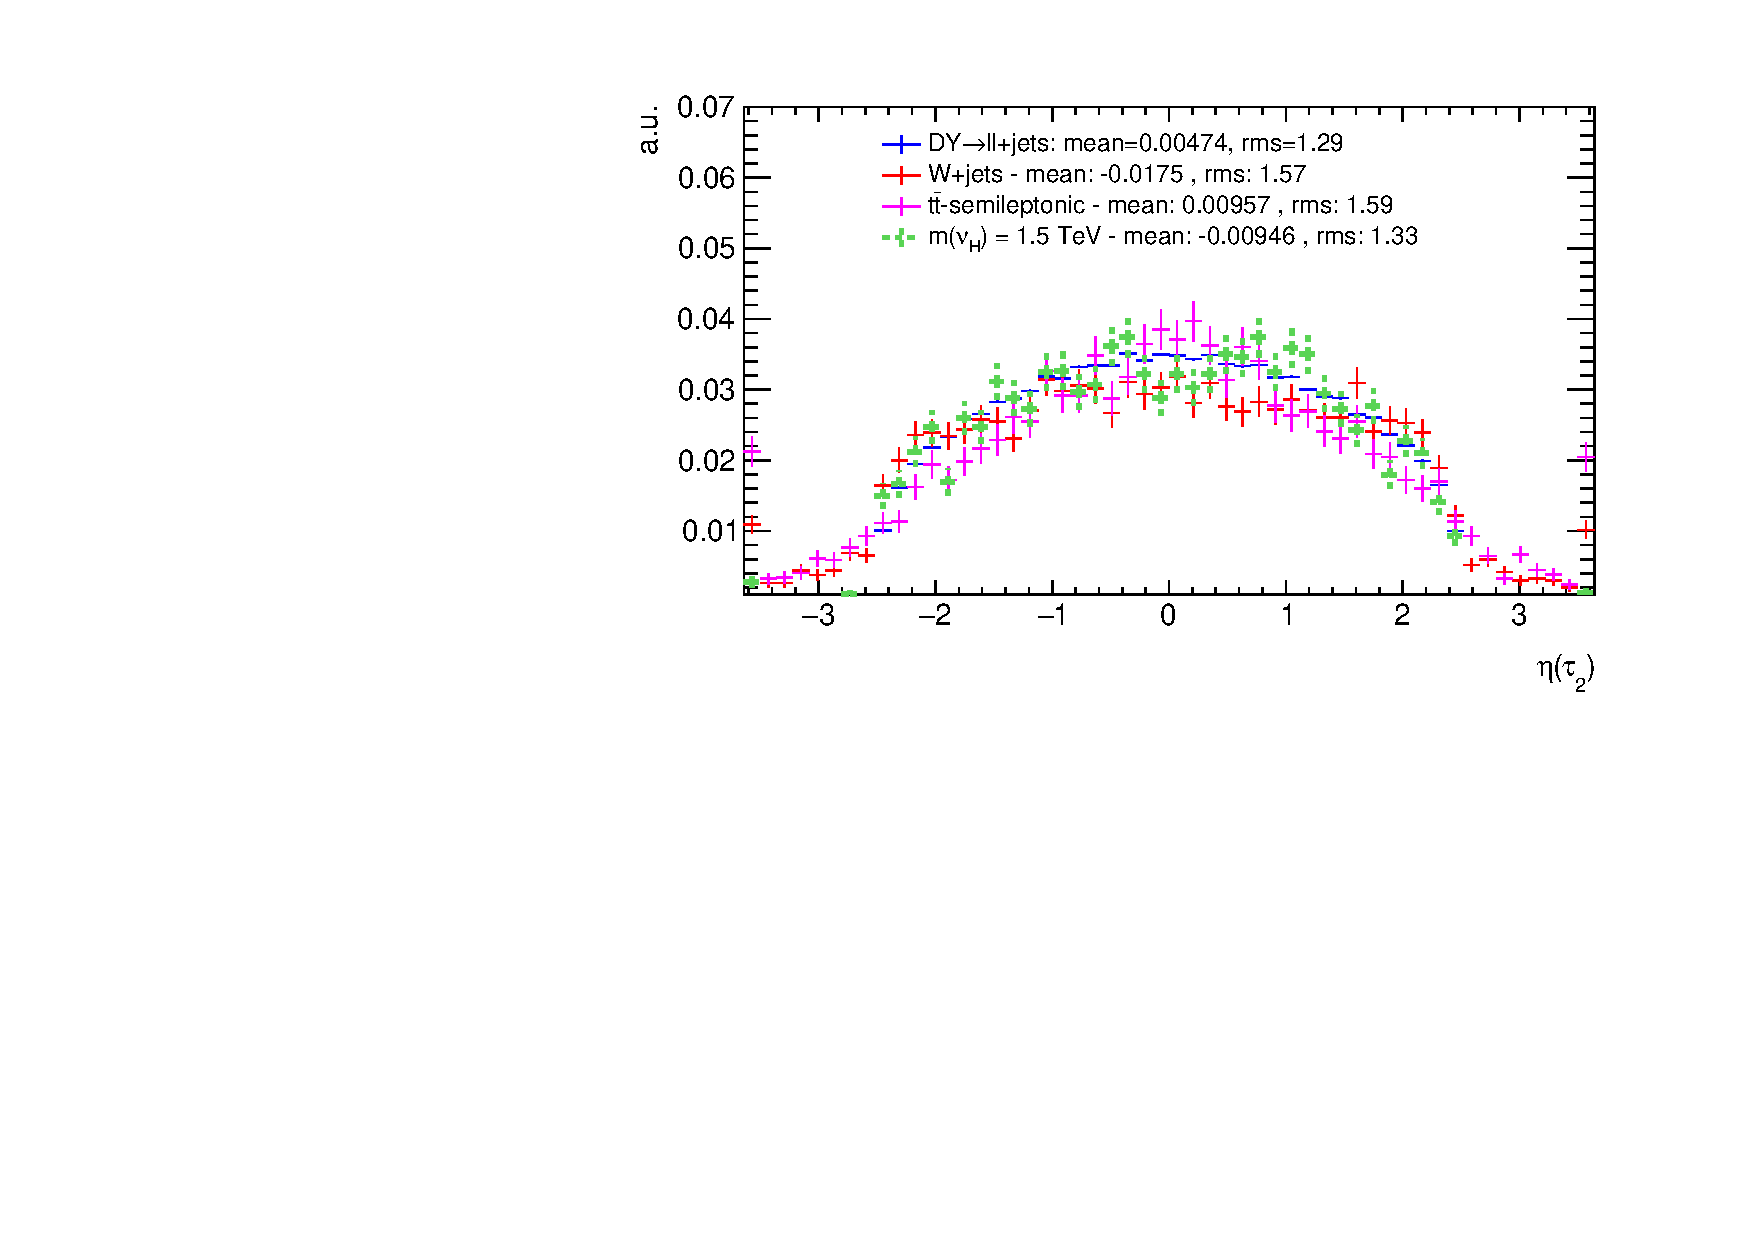
\includegraphics[width=\linewidth]{Plots/tau2_eta_unitNC.pdf}
\caption{Unit plot of $\eta$ from the sub-leading $\tau$ with no cuts}
\label{fig: tau2etaunitNC}
\end{figure}

\begin{figure}
\centering
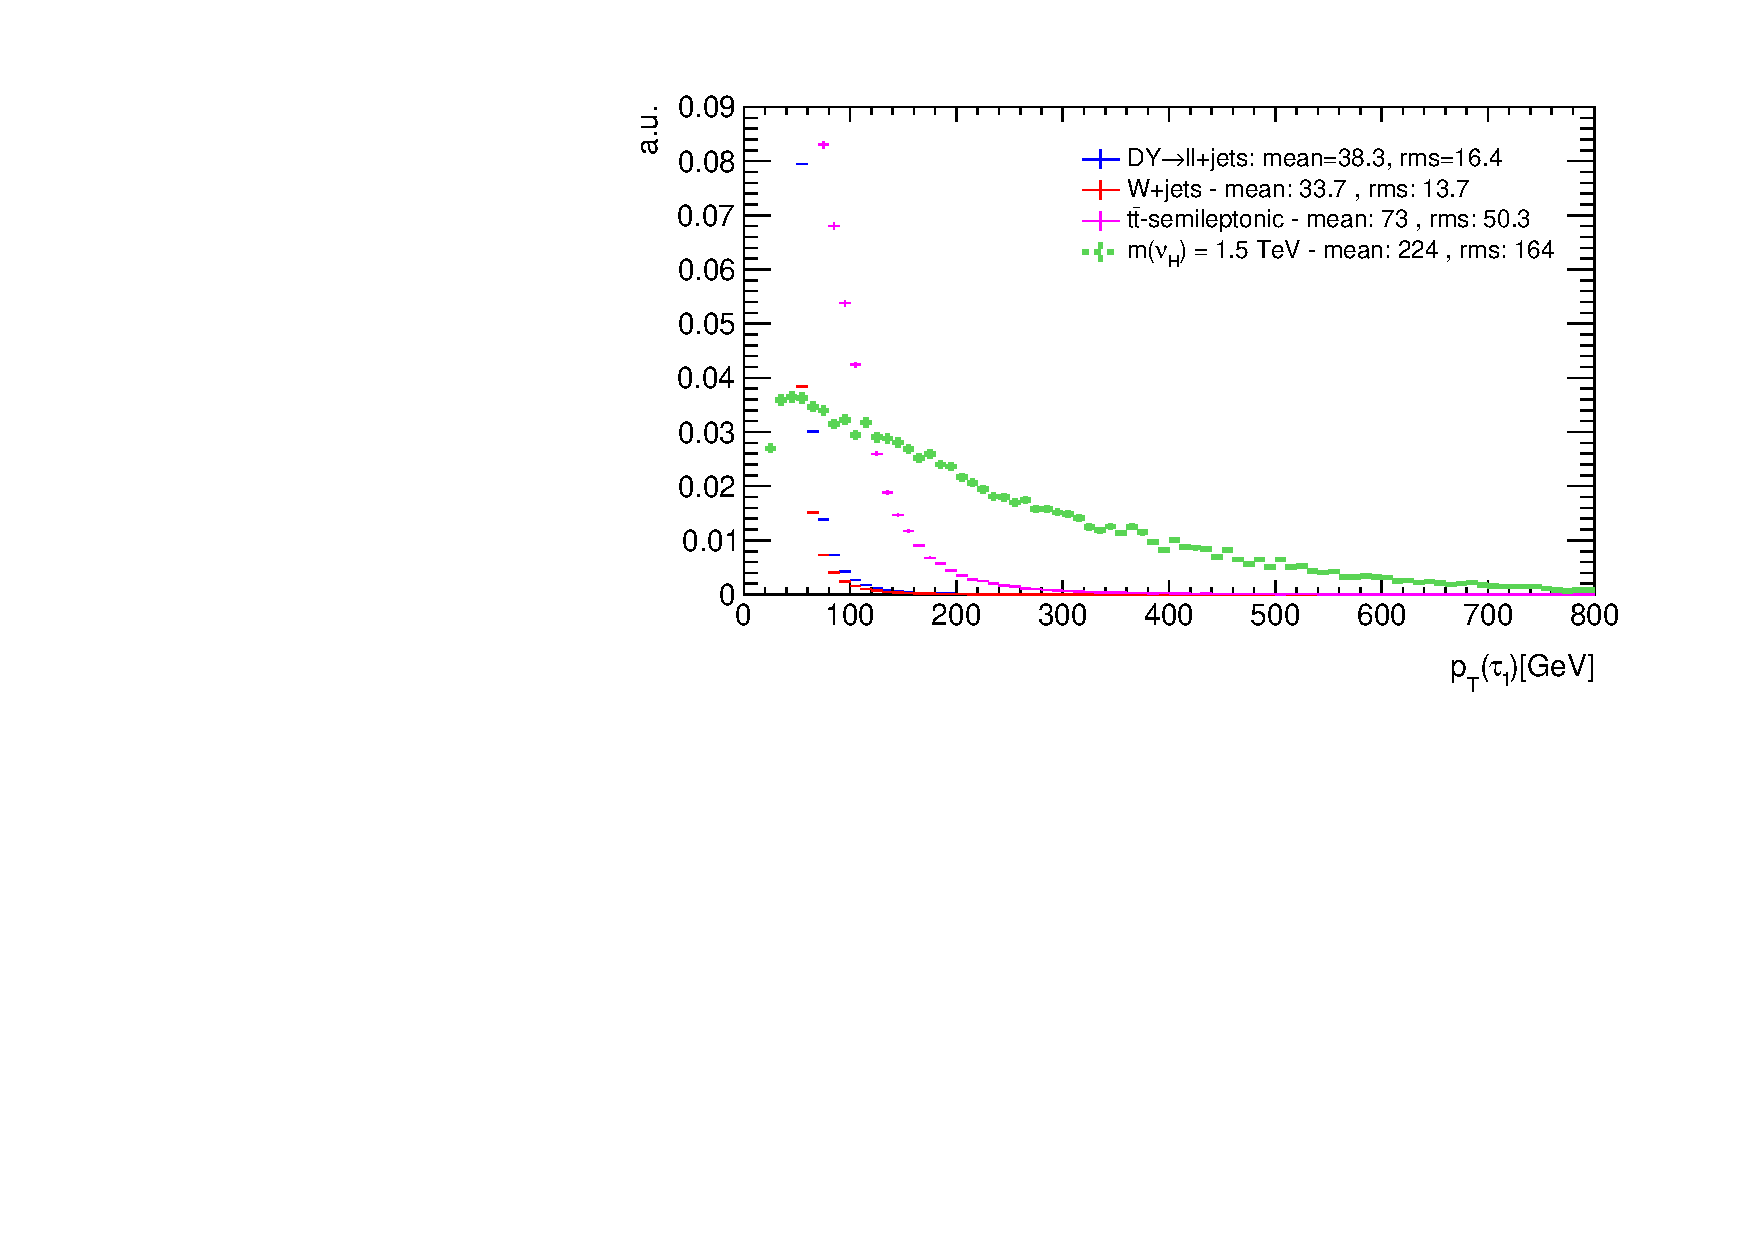
\includegraphics[width=\linewidth]{Plots/tau1_pt_unitNC.pdf}
\caption{Unit plot of $p_{T}$ of leading $\tau$ with no cuts}
\label{fig: tau1ptunitNC}
\end{figure}

To understand the definition of $H_{T}$ and $S_{T}$ mentioned in Chapter \ref{sec:definitions}, the plots in Figure \ref{fig: ptUnitPlots} are shown. The four plots show a separation, in some cases a smaller than others, between the signal and backgrounds distributions. A tendency of the signal jets to have greater transverse momentum than the ones in the backgrounds is shown. This tendency is also displayed for both $\tau$'s. Hence, the distributions of $H_{T}$ and $S_{T}$ should show a similar behaviour because this variables are the result of adding the transverse momentum of jets and $\tau$'s in the event.

\begin{figure}       
        \centering
        \begin{subfigure}[b]{0.475\textwidth}
            \centering
            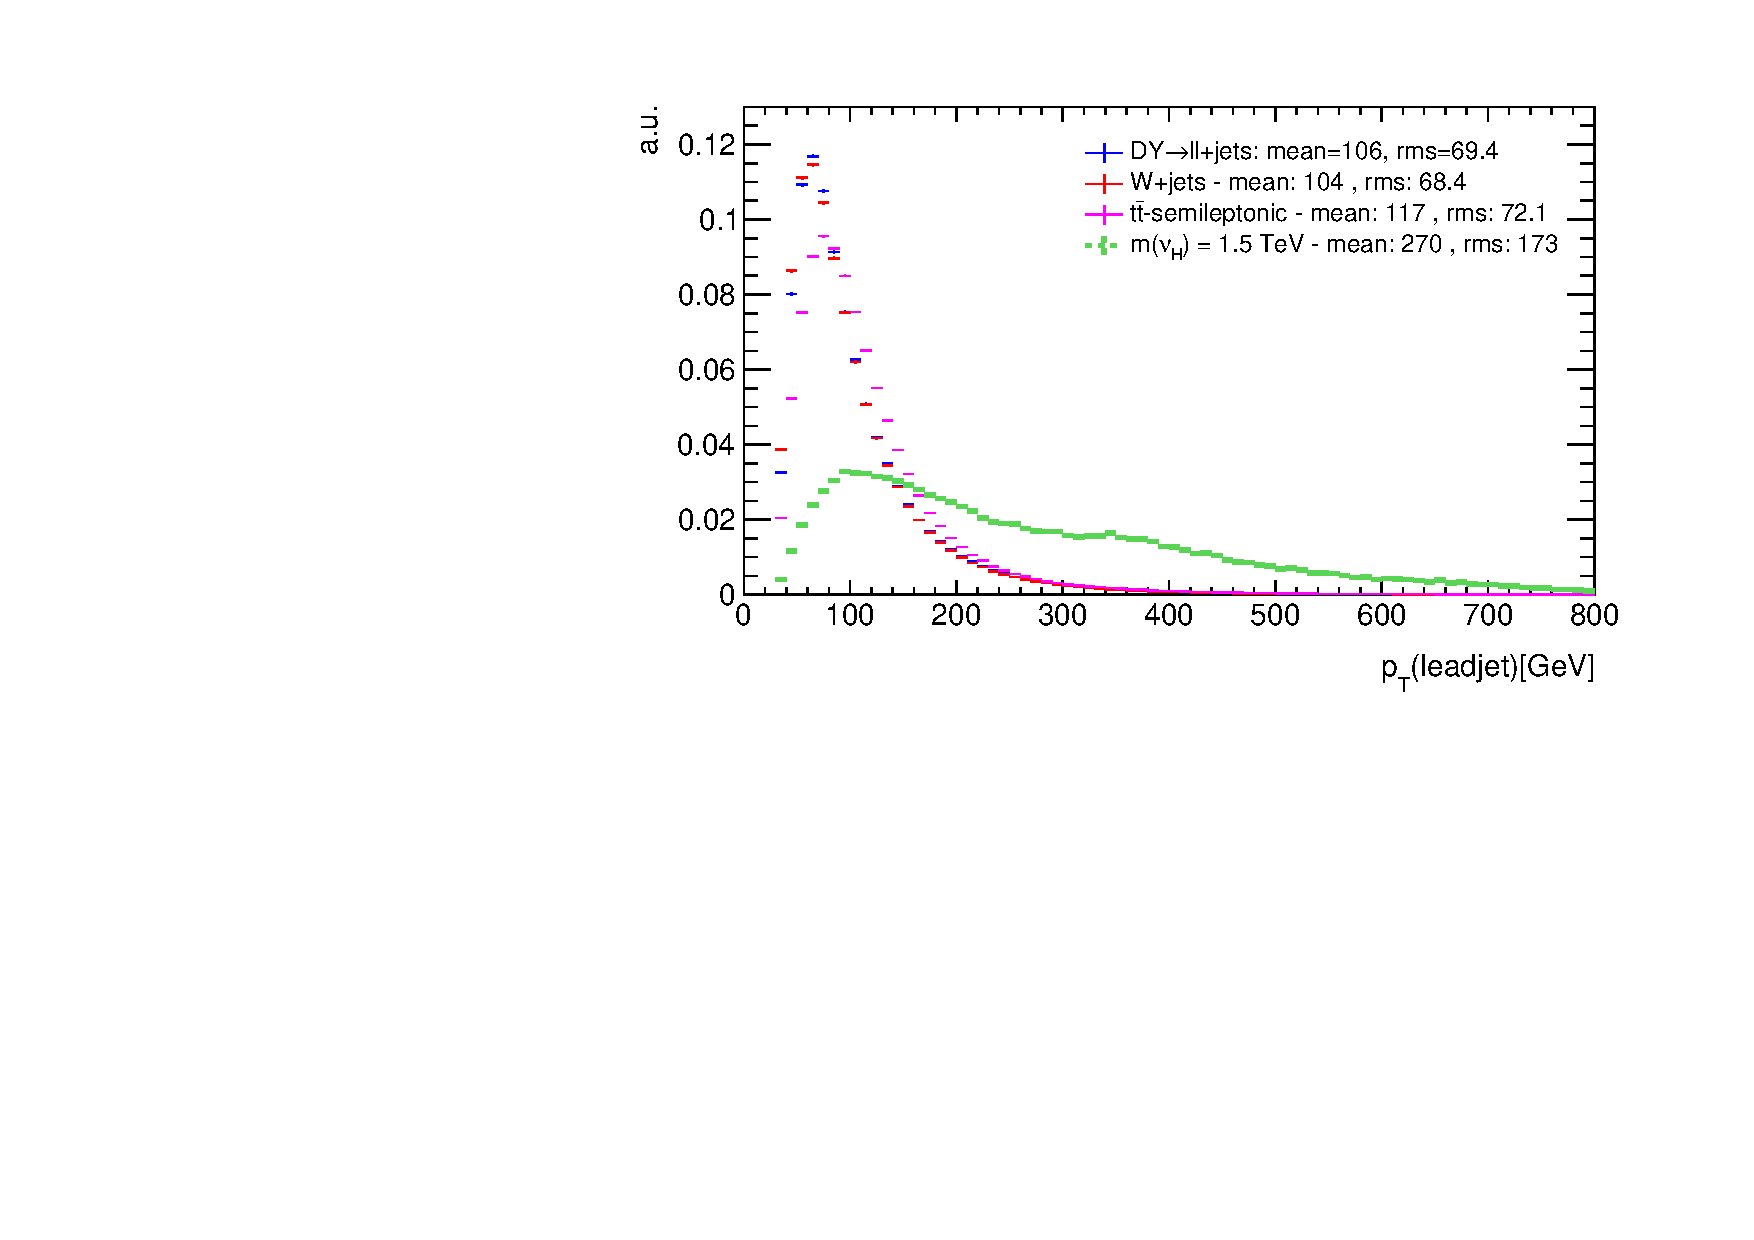
\includegraphics[width=\textwidth]{Plots/ljet_pt_unitNC}
            \caption[]%
            {{\small Leading jet $p_{T}$ unit plot}}    
            %\label{fig:mean and std of net14}
        \end{subfigure}
        \hfill
        \begin{subfigure}[b]{0.475\textwidth}  
            \centering 
            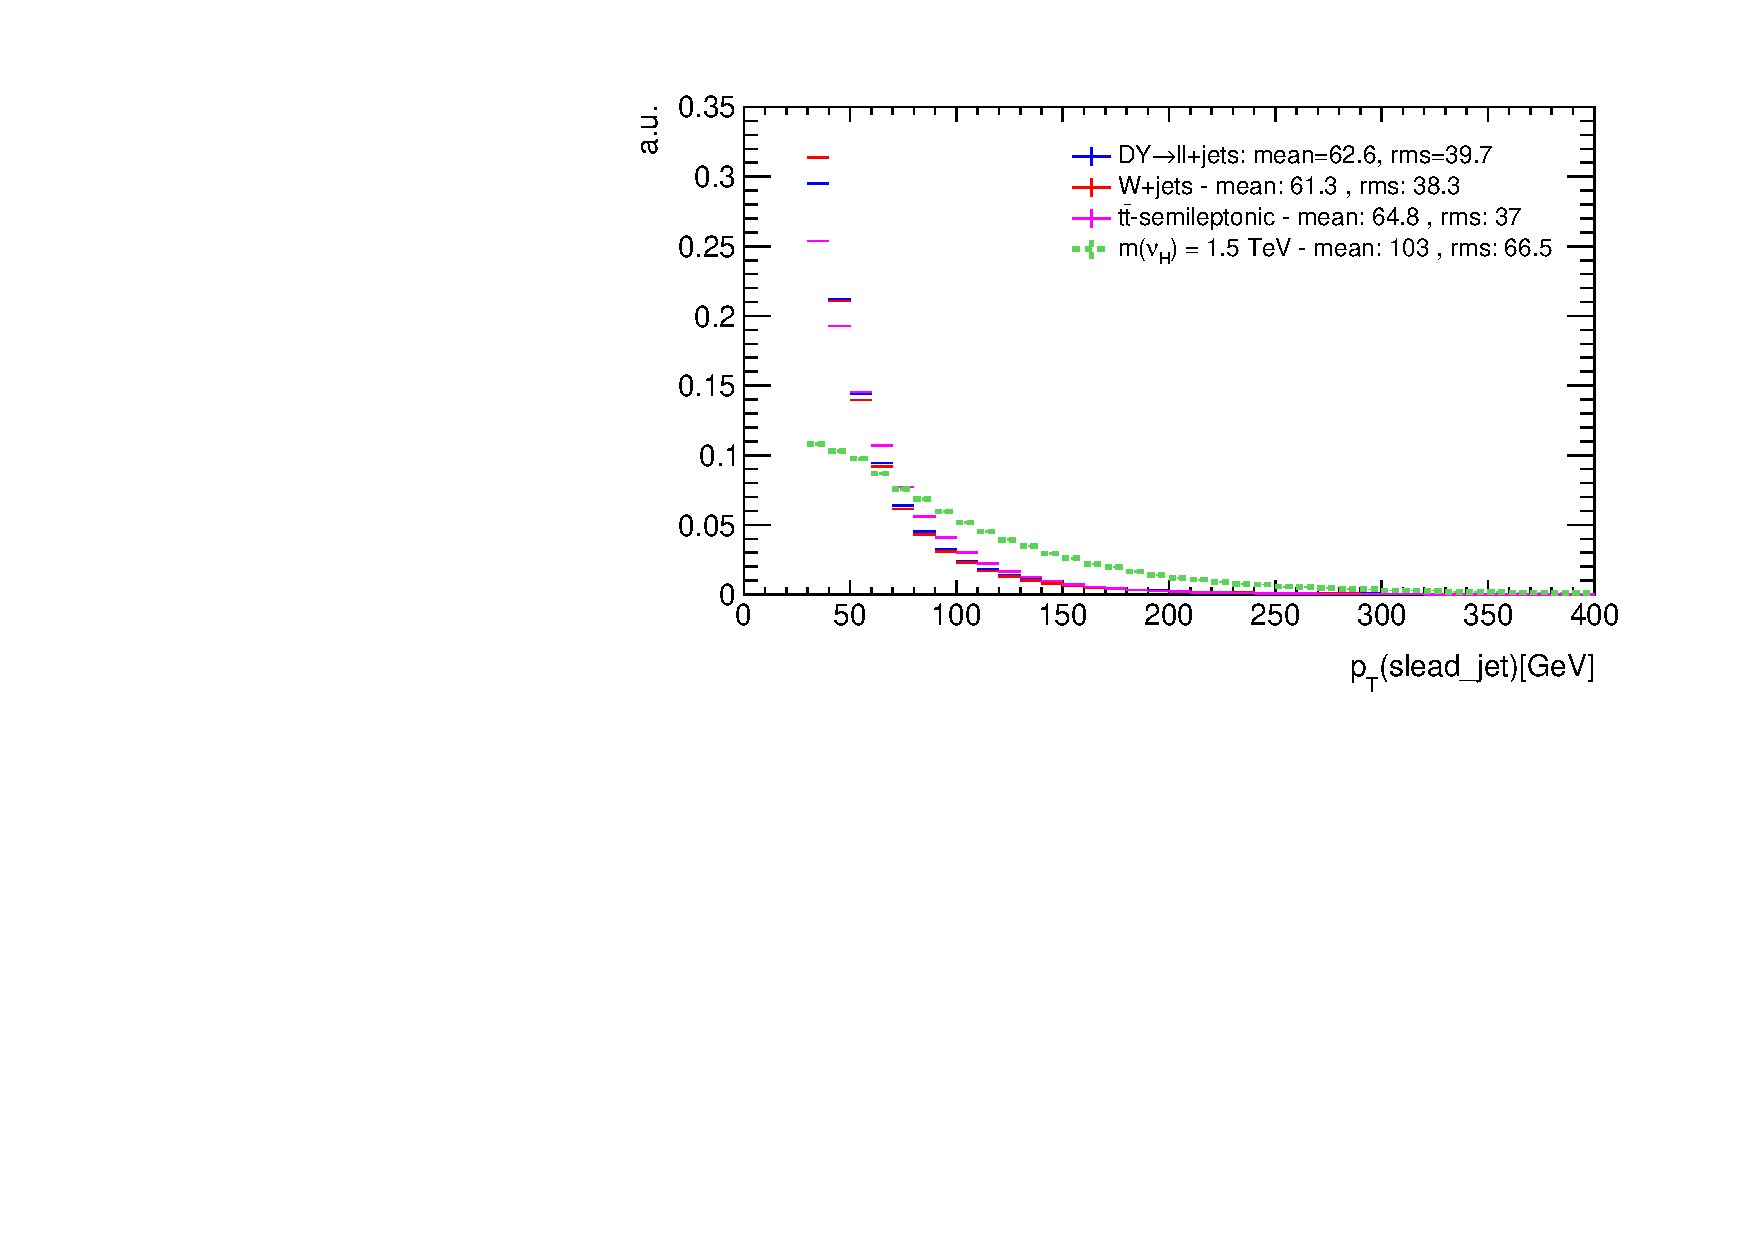
\includegraphics[width=\textwidth]{Plots/sjet_pt_unitNC}
            \caption[]%
            {{\small Sub-leading jet $p_{T}$ unit plot}}    
            %\label{fig:mean and std of net24}
        \end{subfigure}
        \vskip\baselineskip
        \begin{subfigure}[b]{0.475\textwidth}   
            \centering 
            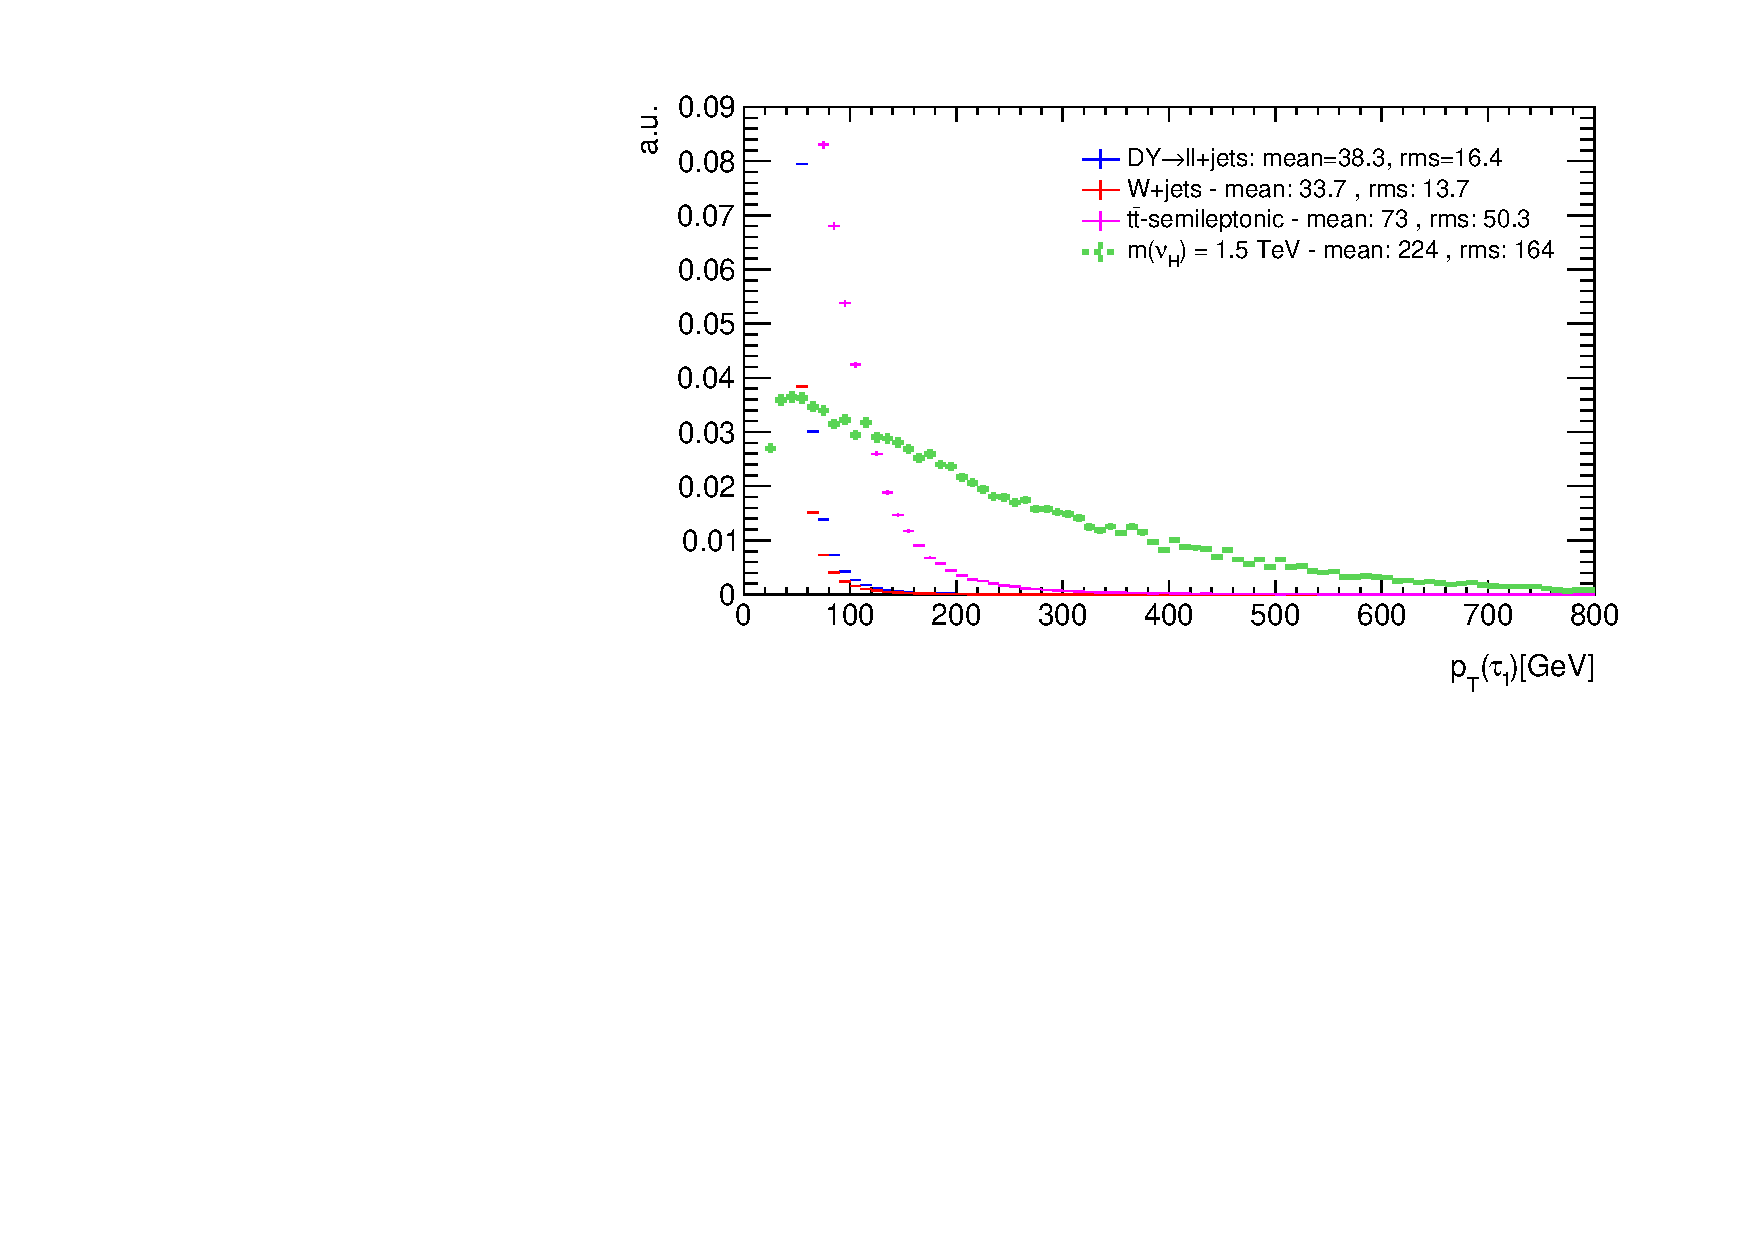
\includegraphics[width=\textwidth]{Plots/tau1_pt_unitNC}
            \caption[]%
            {{\small Leading $\tau$ $p_{T}$ unit plot}}    
            %\label{fig:mean and std of net34}
        \end{subfigure}
        \quad
        \begin{subfigure}[b]{0.475\textwidth}   
            \centering 
            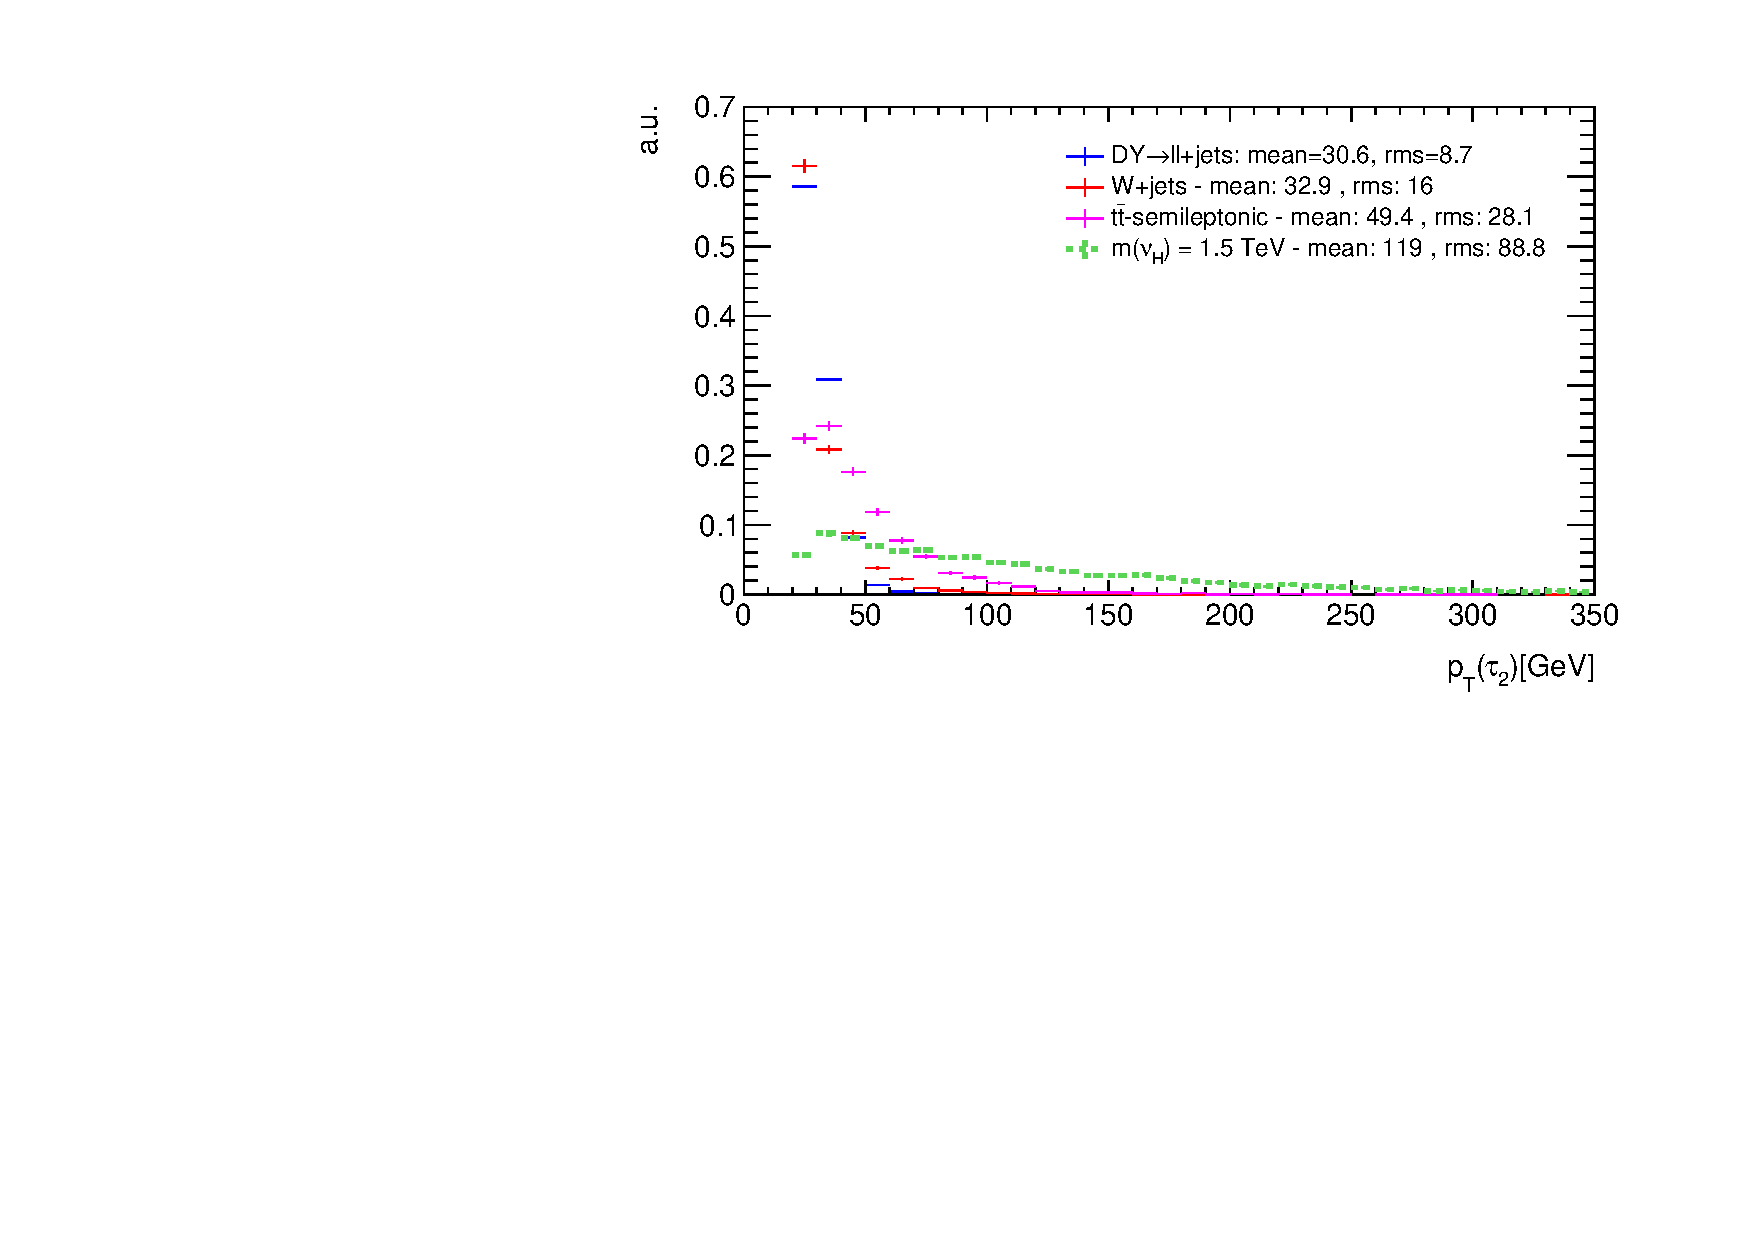
\includegraphics[width=\textwidth]{Plots/tau2_pt_unitNC}
            \caption[]%
            {{\small Sub-leading $\tau$ $p_{T}$ unit plot}}    
            %\label{fig:mean and std of net44}
        \end{subfigure}
        \caption[ $p_T$ unit plots for different bodies in the event]
        {\small $p_T$ unit plots for different bodies in the event} 
         \label{fig: ptUnitPlots}
\end{figure}

In Figures \ref{fig: HTunitNC} and \ref{fig: STunitNC}, the normalized plots with no cuts of $H_{T}$ and $S_{T}$ are shown. It can be seen that indeed a greater separation between signal and background was achieved. Unlike the distributions of the $\tau$'s and jets transverse momentum, the maxima of $H_{T}$ and $S_{T}$ lie outside the backgrounds distributions. Furthermore, the background that overlaps at a greater energy with the signal corresponds to $t\bar{t}$. Taking into account what was mentioned in section \ref{sec: cutdefinitions}, the overlap between the signal and this background could be reduced with the cut related with the number of B-jets in the event. This is why this two variables need to be studied closer in the analysis.

\begin{figure}
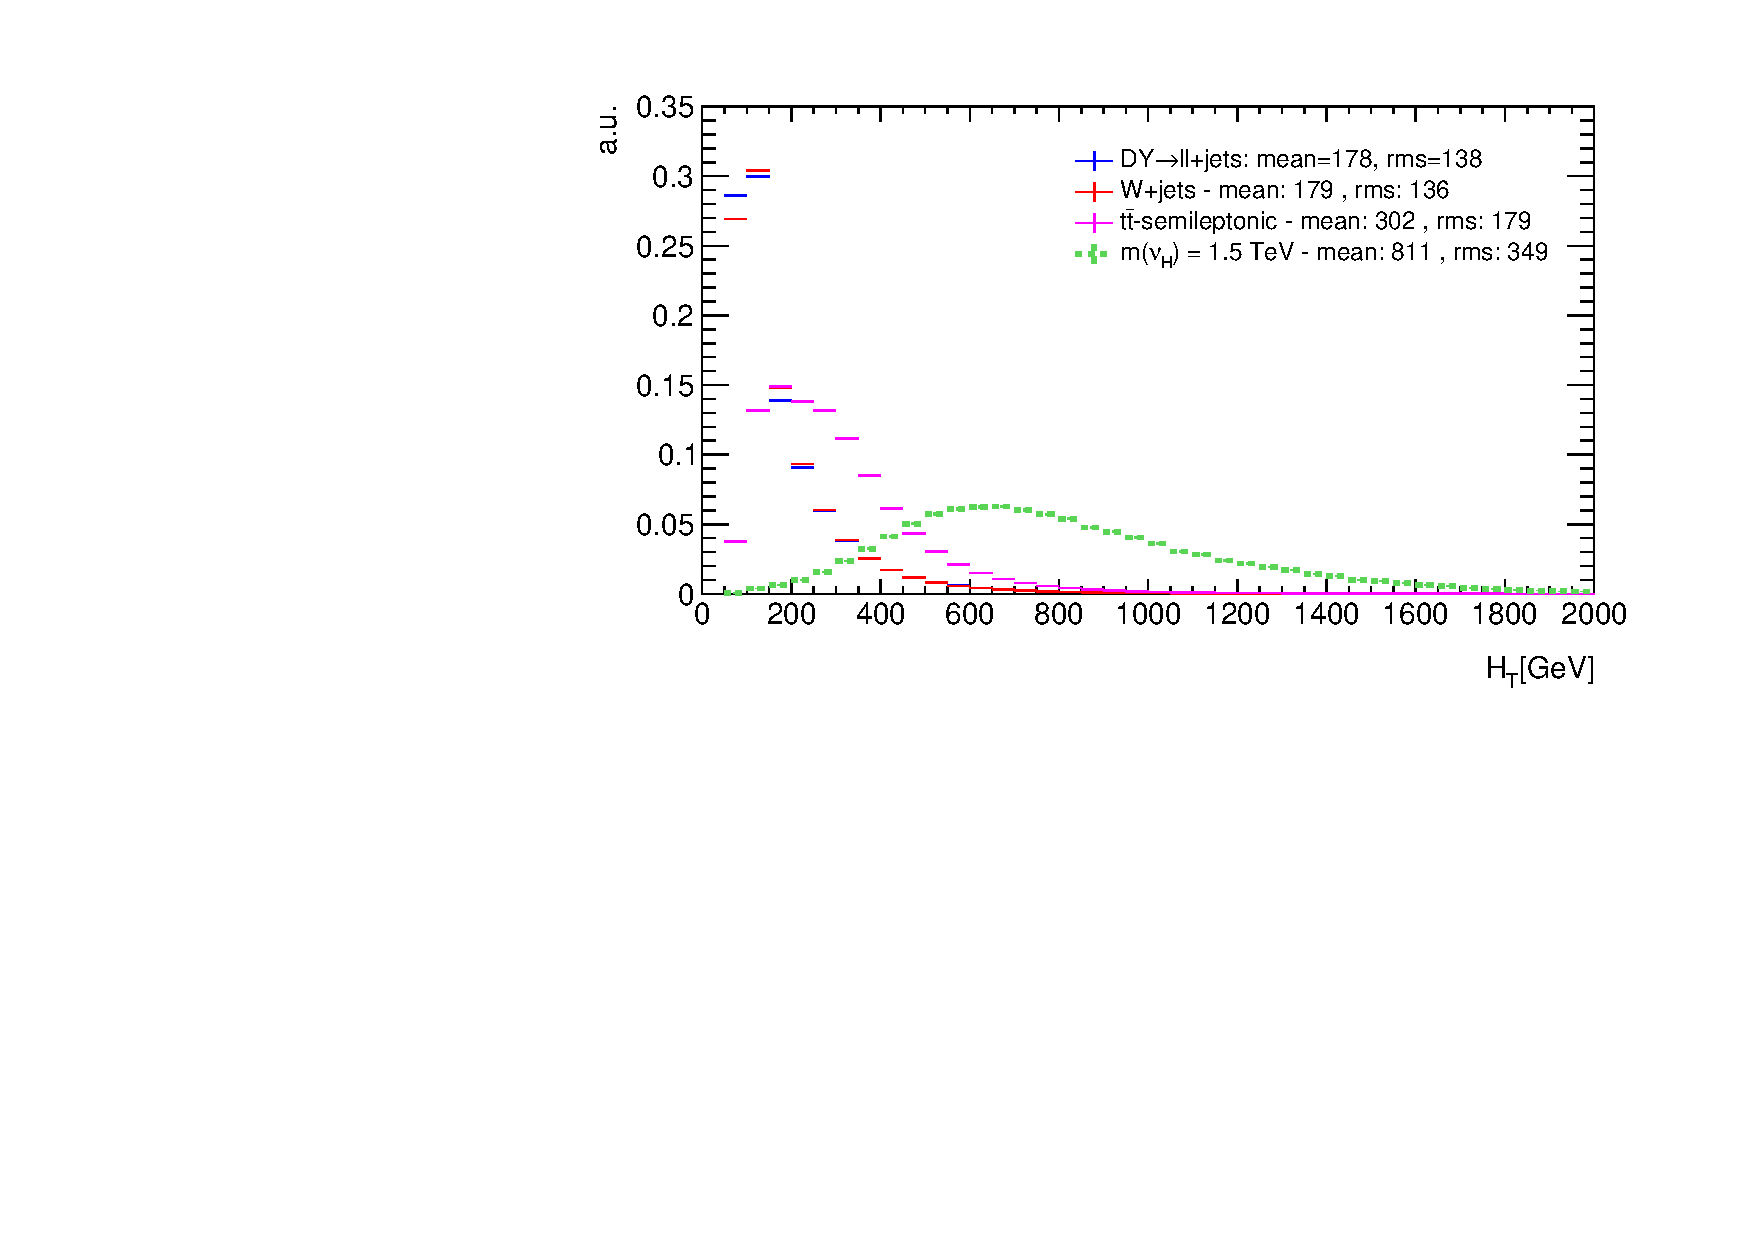
\includegraphics[width=\linewidth]{Plots/HT_unitNC.pdf}
\caption{Unit plot of $H_{T}$ with no cuts}
\label{fig: HTunitNC}
\end{figure}

\begin{figure}
\centering
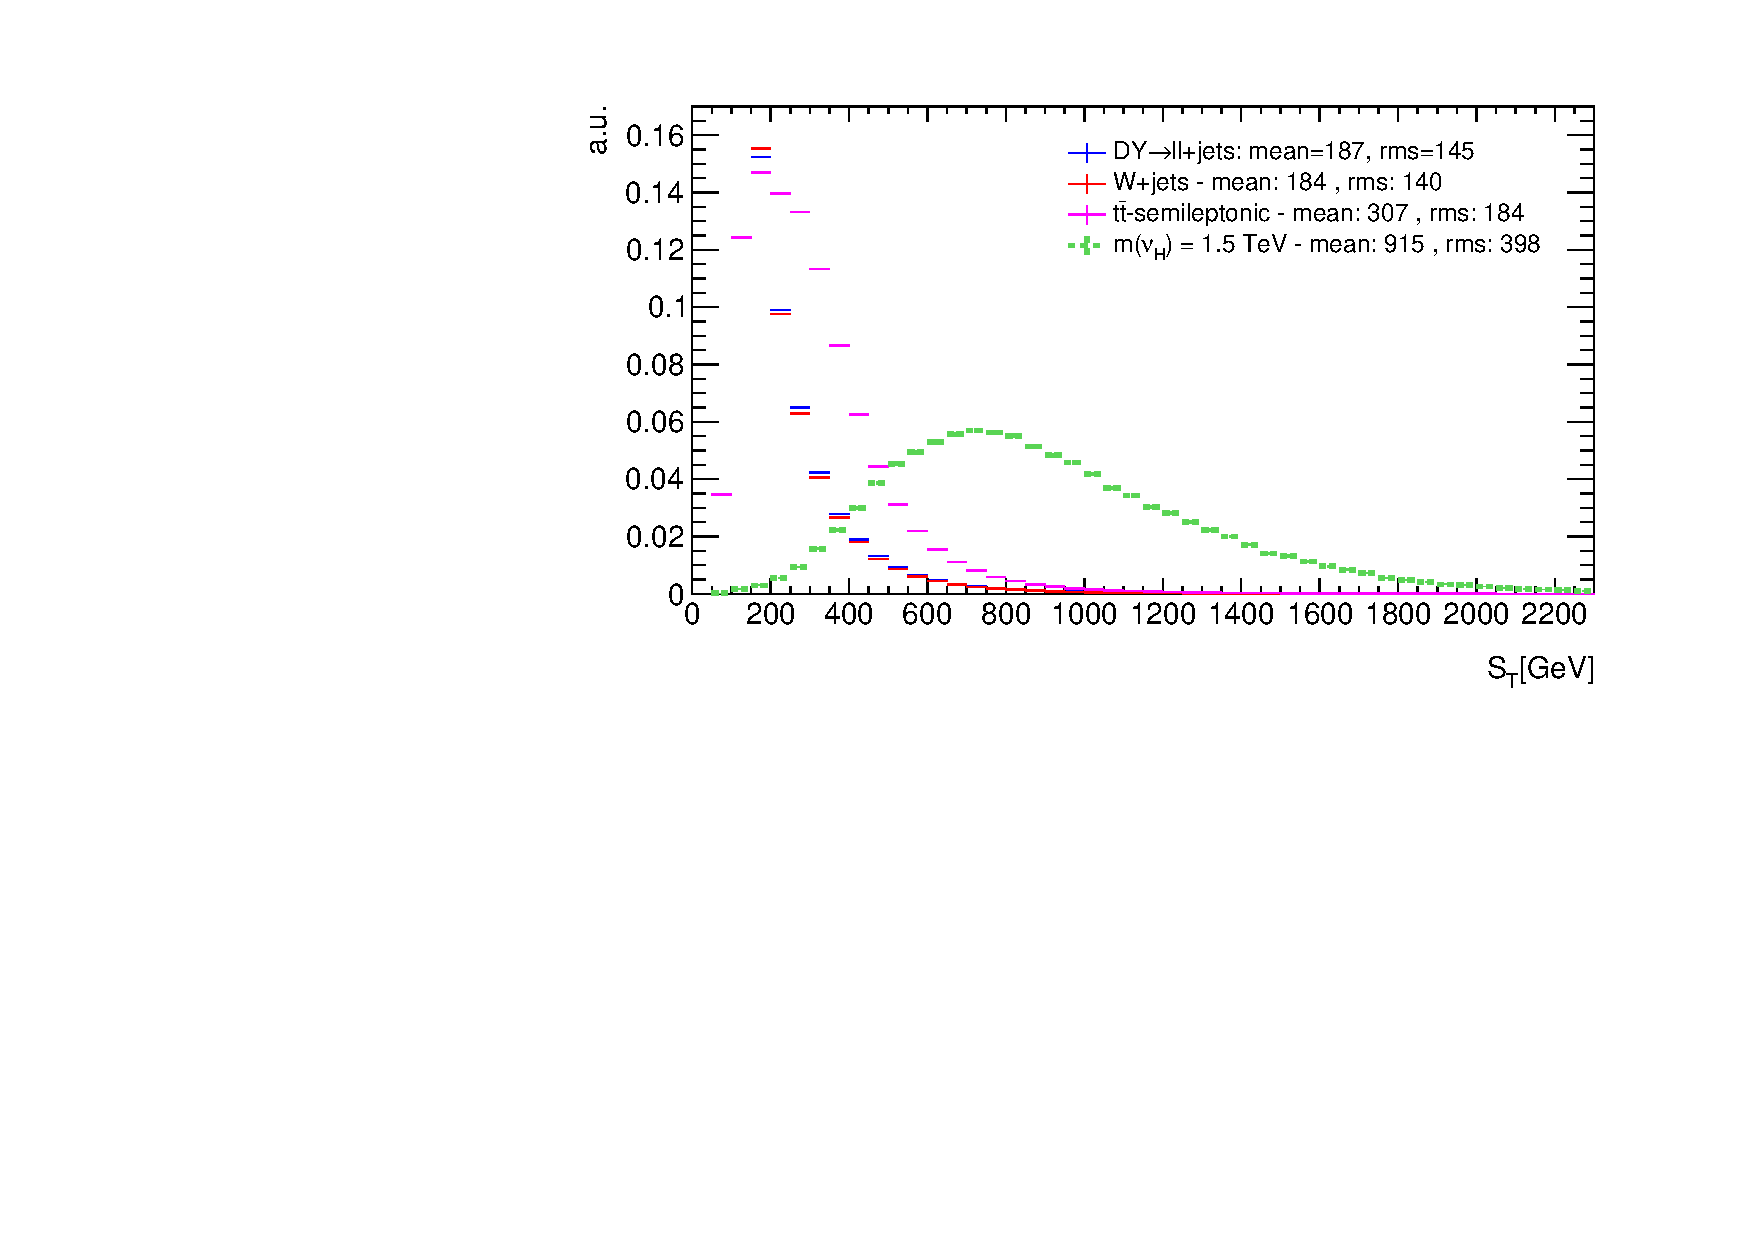
\includegraphics[width=\linewidth]{Plots/ST_unitNC.pdf}
\caption{Unit plot of $S_{T}$ with no cuts}
\label{fig: STunitNC}
\end{figure}

Another variable relevant for the analysis was found out to be $m(jj)$. The reason for a further analysis of this variable is shown in Figure \ref{fig: mjjUnitNC}. As in the case of $H_{T}$ and $S_{T}$, the distribution of the mass of the Di-Jet Pair shows a separation between the signal and the three backgrounds. Furthermore, it shows a greater separation than the one observed for both $H_{T}$ and $S_{T}$. That is why, the variable $m(jj)$, or the total mass of the Di-Jet Pair, has to be studied more closely, because it shows potential for a separation between signal and backgrounds.

\begin{figure}
\centering
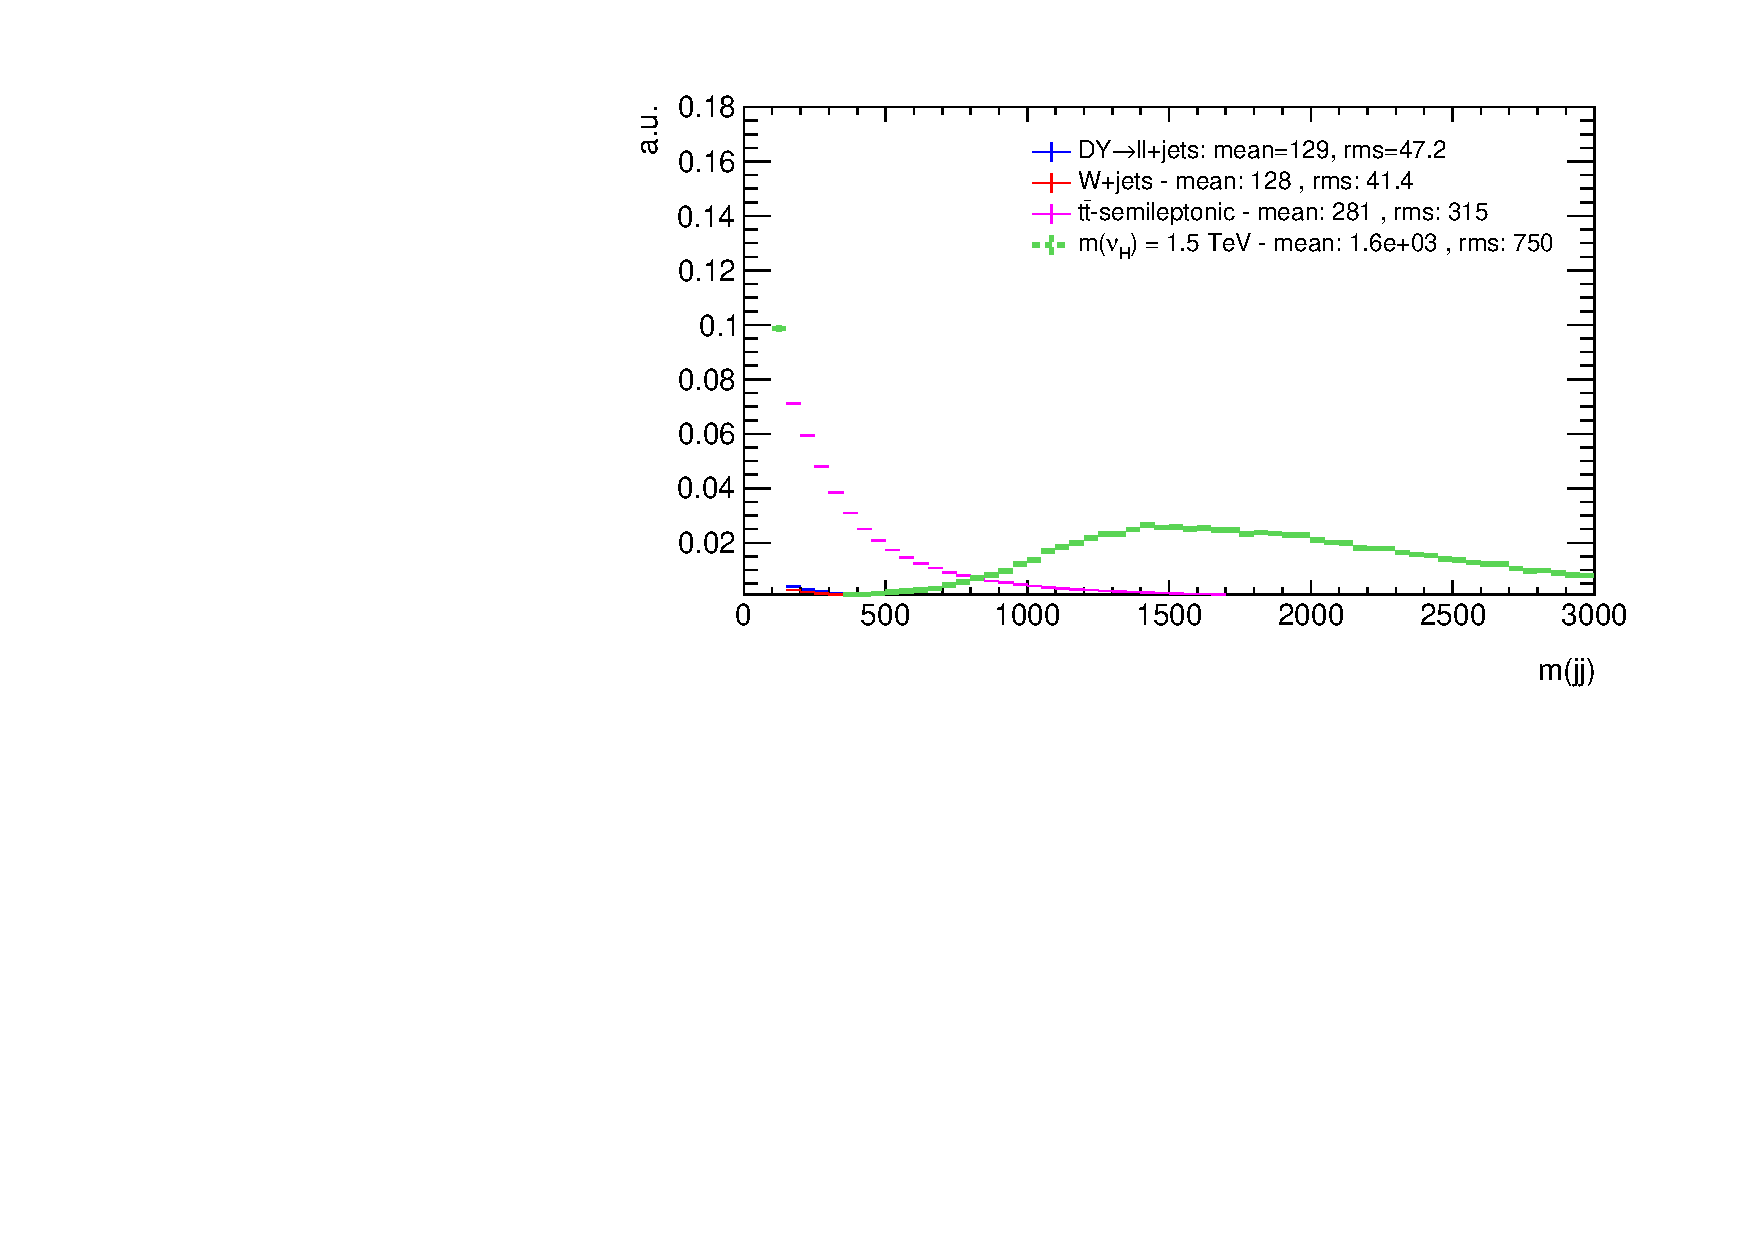
\includegraphics[width=\linewidth]{Plots/mjj_unitNC.pdf}
\caption{Unit plot of $m(jj)$ with no cuts}
\label{fig: mjjUnitNC}
\end{figure}

In Figures \ref{fig: HTunitVBF} and \ref{fig: STunitVBF}, the plots incuding cuts of $H_{T}$ and $S_{T}$ respectively are shown. Both plots include all the cuts mentioned in section \ref{sec: selectionCriteria}. A rebining of the histograms was necessary, because due to the cuts, the number of backgrounds events decreased significantly. This made the error bars for these histograms larger making the analysis of the plot more difficult. For that reason, a bin size of 400 GeV was defined for both of these plots. Comparing the two signal histograms, it can be seen that the maximum of the $H_{T}$ distribution still overlaps with the background distributions. Although the signal in this case appears on top of the background, it has to be noted that this normalized plots are only useful to get an idea of the distribution shapes. That is why the fact the the signal appears on top of the background does not mean that the signal can be detected over the background for this value. On the contrary, the maximum of the $S_{T}$ signal distribution has its maximum when the background distributions start to decay. This distribution shape  difference between $H_{T}$ and $S_{T}$ is related with the fact that the signal has $\tau$'s with higher $p_{T}$ than the ones found in the backgrounds.

\begin{figure}
\begin{center}
 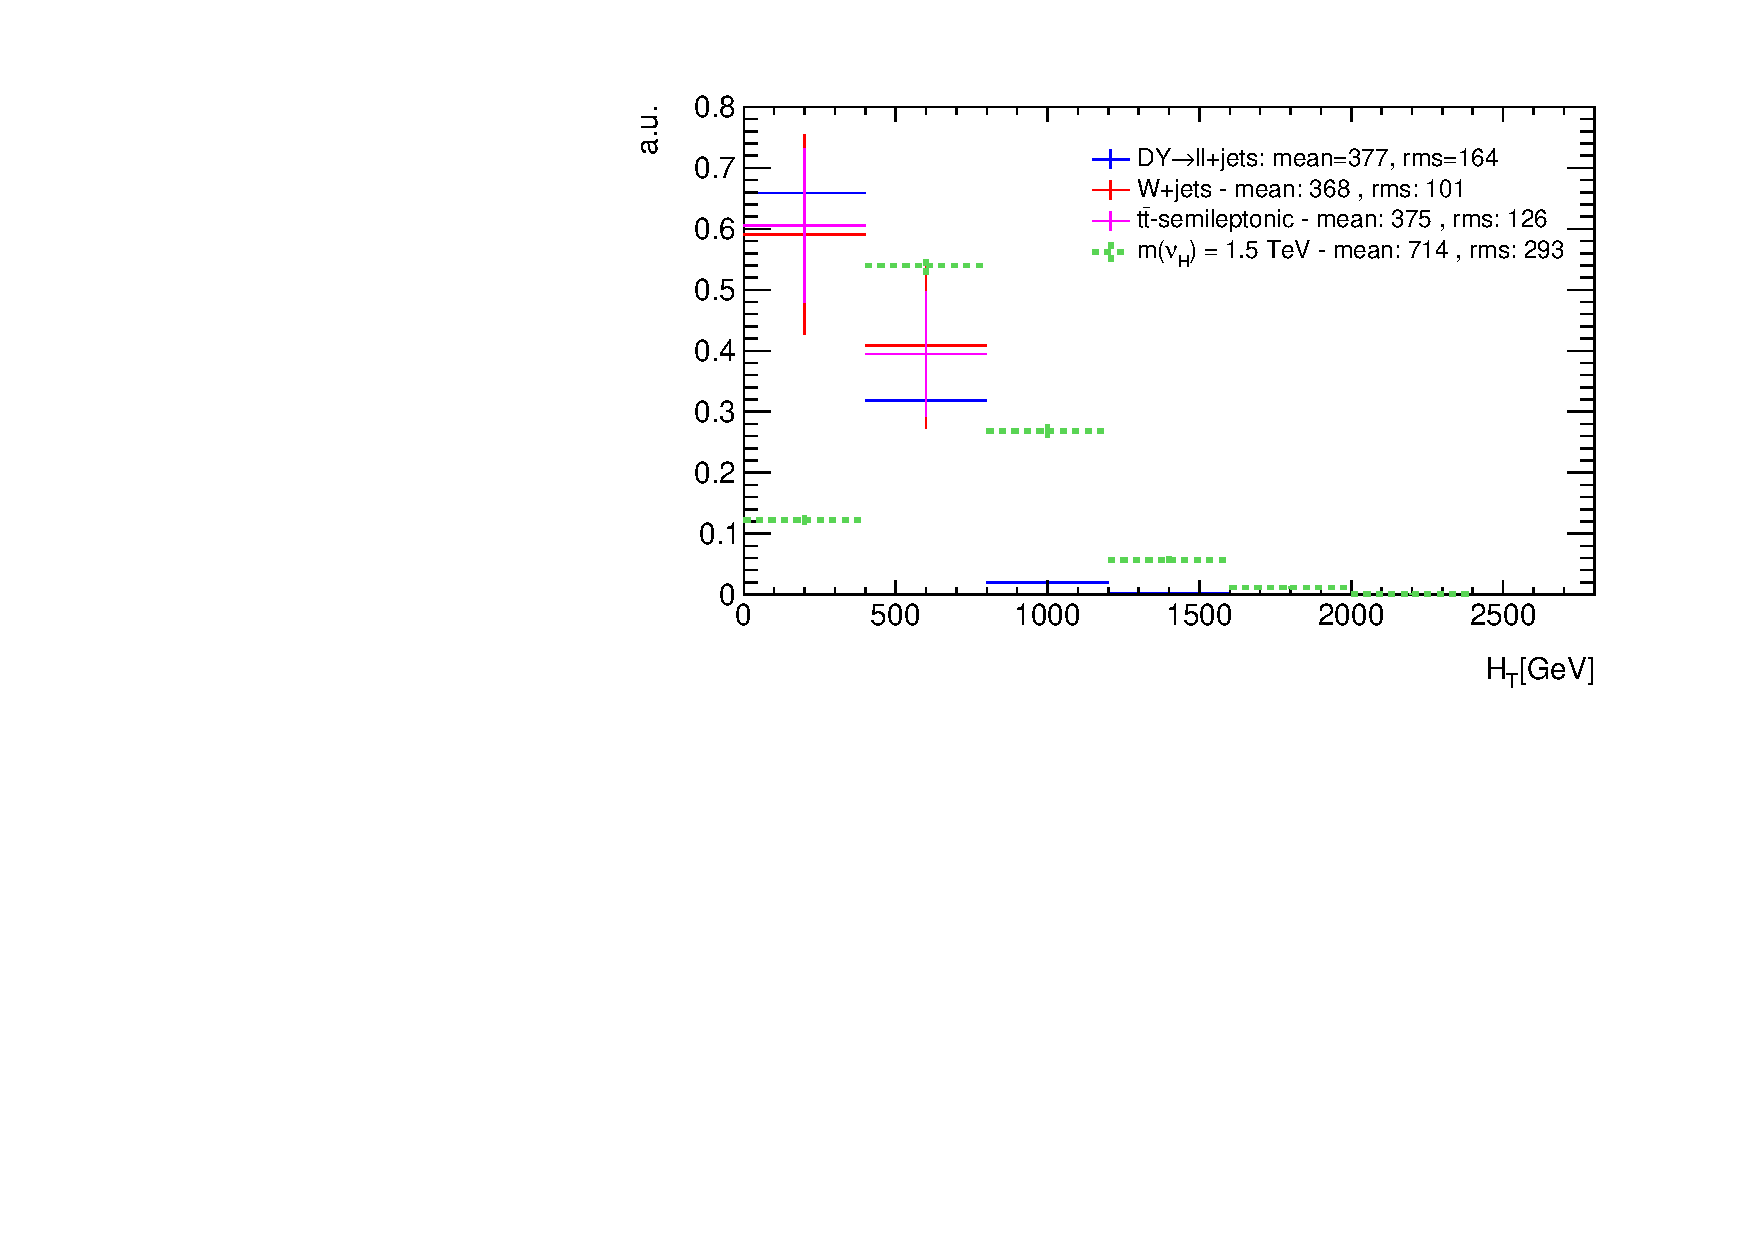
\includegraphics[width=\linewidth]{Plots/HT_unitVBF.pdf}
\end{center}
\caption{Unit plot of $H_{T}$ with VBF cuts}
\label{fig: HTunitVBF}
\end{figure}

\begin{figure}
\centering
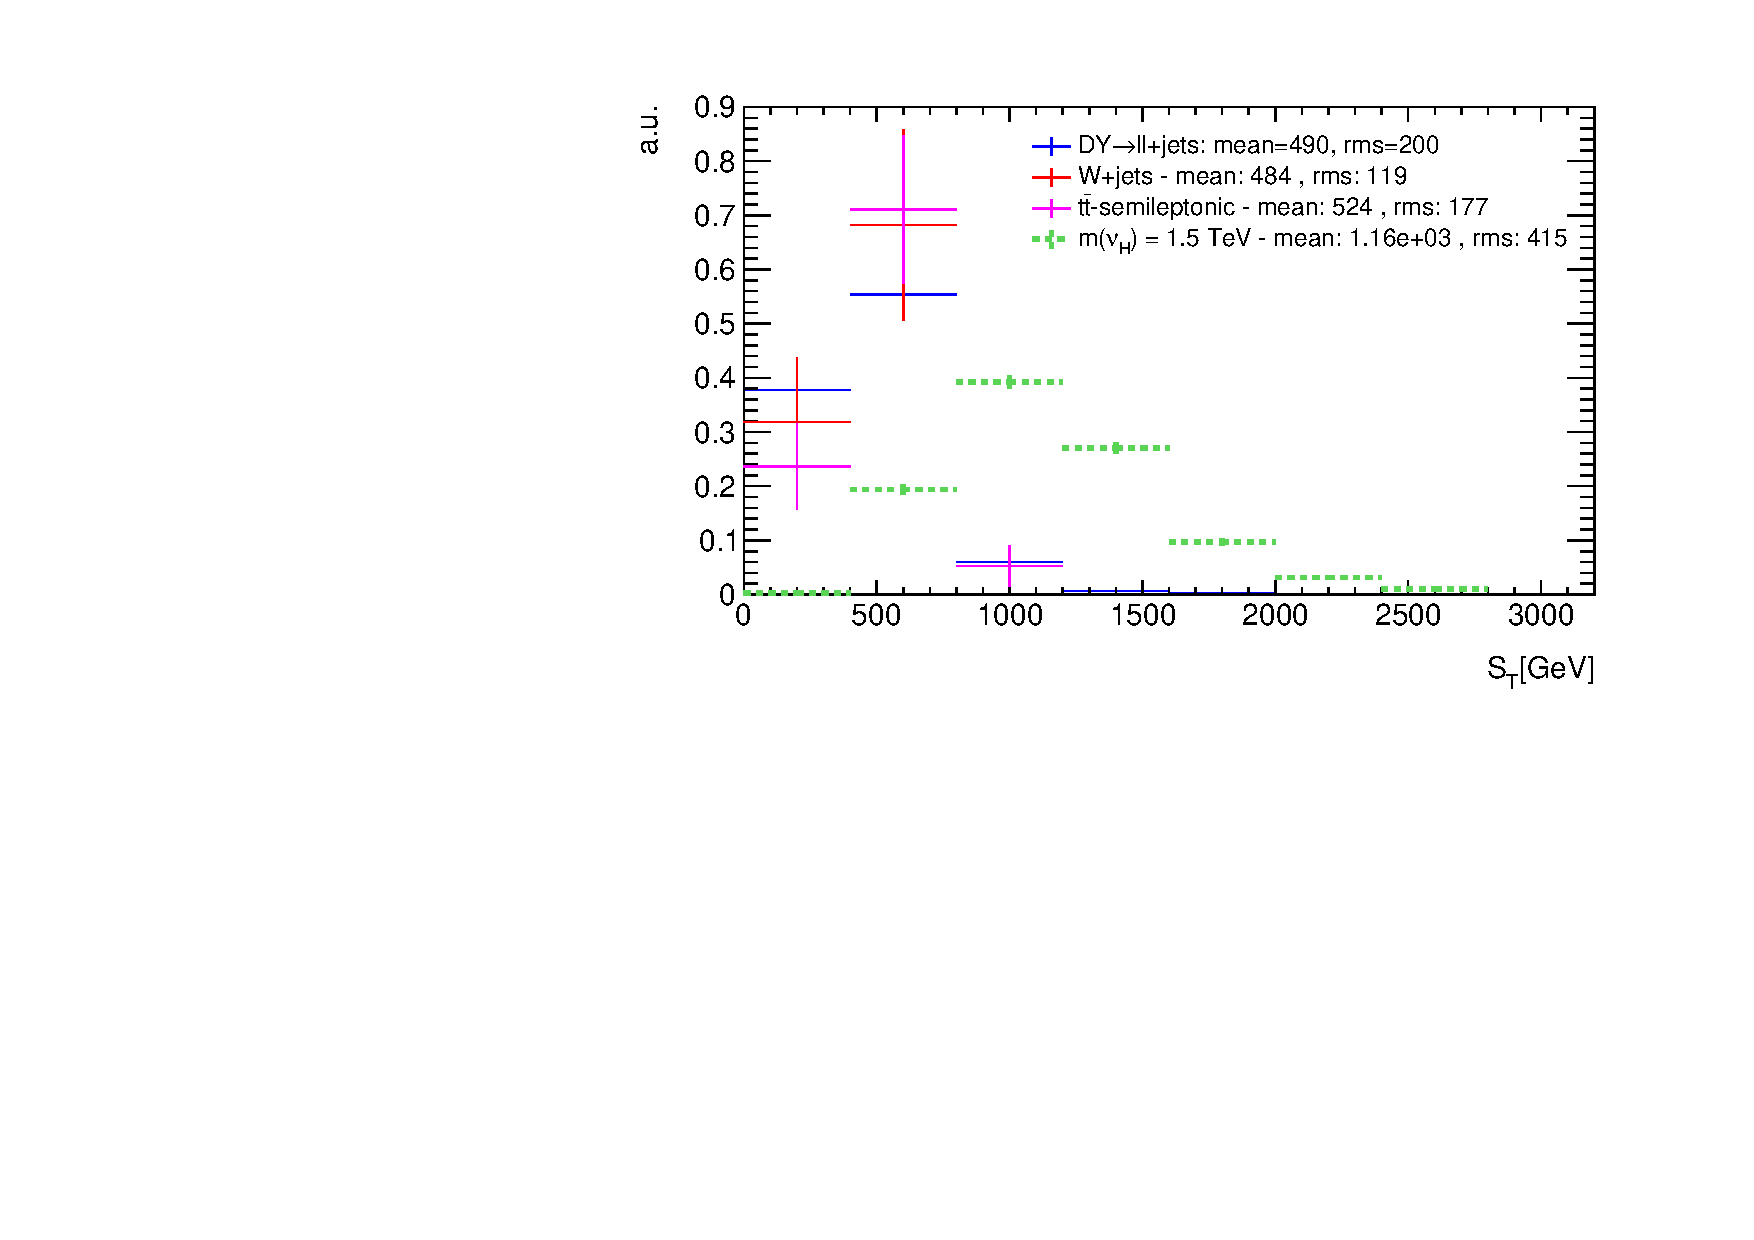
\includegraphics[width=\linewidth]{Plots/ST_unitVBF.pdf}
\caption{Unit plot of $S_{T}$ with VBF cuts}
\label{fig: STunitVBF}
\end{figure}

The mean values for $S_{T}$ shown in Figures \ref{fig: STunitNC} and \ref{fig: STunitVBF} are 915 GeV and 1160 GeV respectively. From the Feynman diagram in Figure \ref{fig: hnGamma}, it can be seen that the jets in the event and one of the taus come from the heavy neutrino decay. Taking into account that the defined mass for the heavy neutrino is 1.5 TeV, it is expected that the maximum of the $S_{T}$ distribution is around this value. This analysis leads to the conclusion that the cuts made to the histograms are helping to select the significant events, because the mean $S_{T}$ is closer to the expected value after performing all the cuts.

\section{Stack Plots}

\begin{figure}
\centering
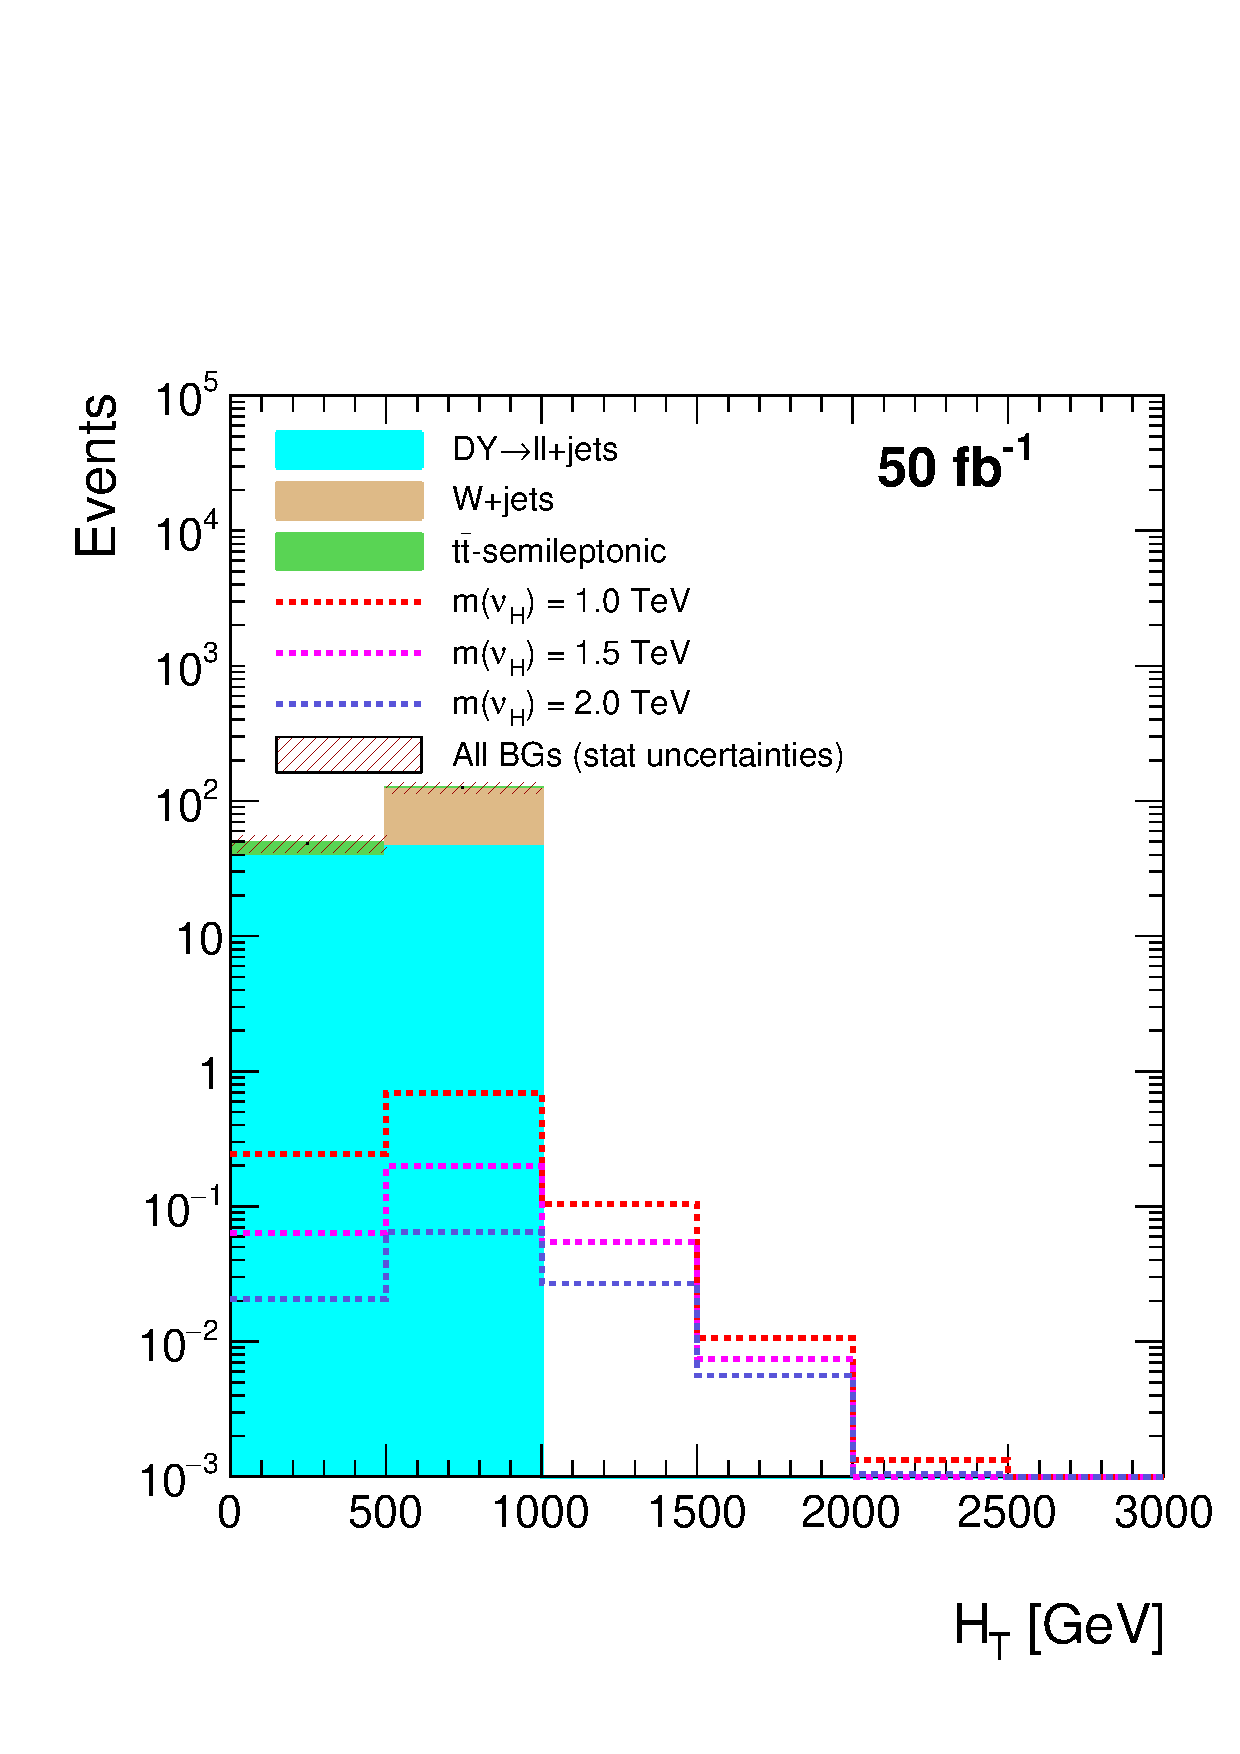
\includegraphics[width=\linewidth]{StackPlots/HT_2taus_met50_50ifb.pdf}
\caption{Stack plot of $H_{T}$ requiring two taus in the event and with $\slashed{E}_{T} > 50$}
\label{fig: HT2tausMet50}
\end{figure}

\begin{figure}
\centering
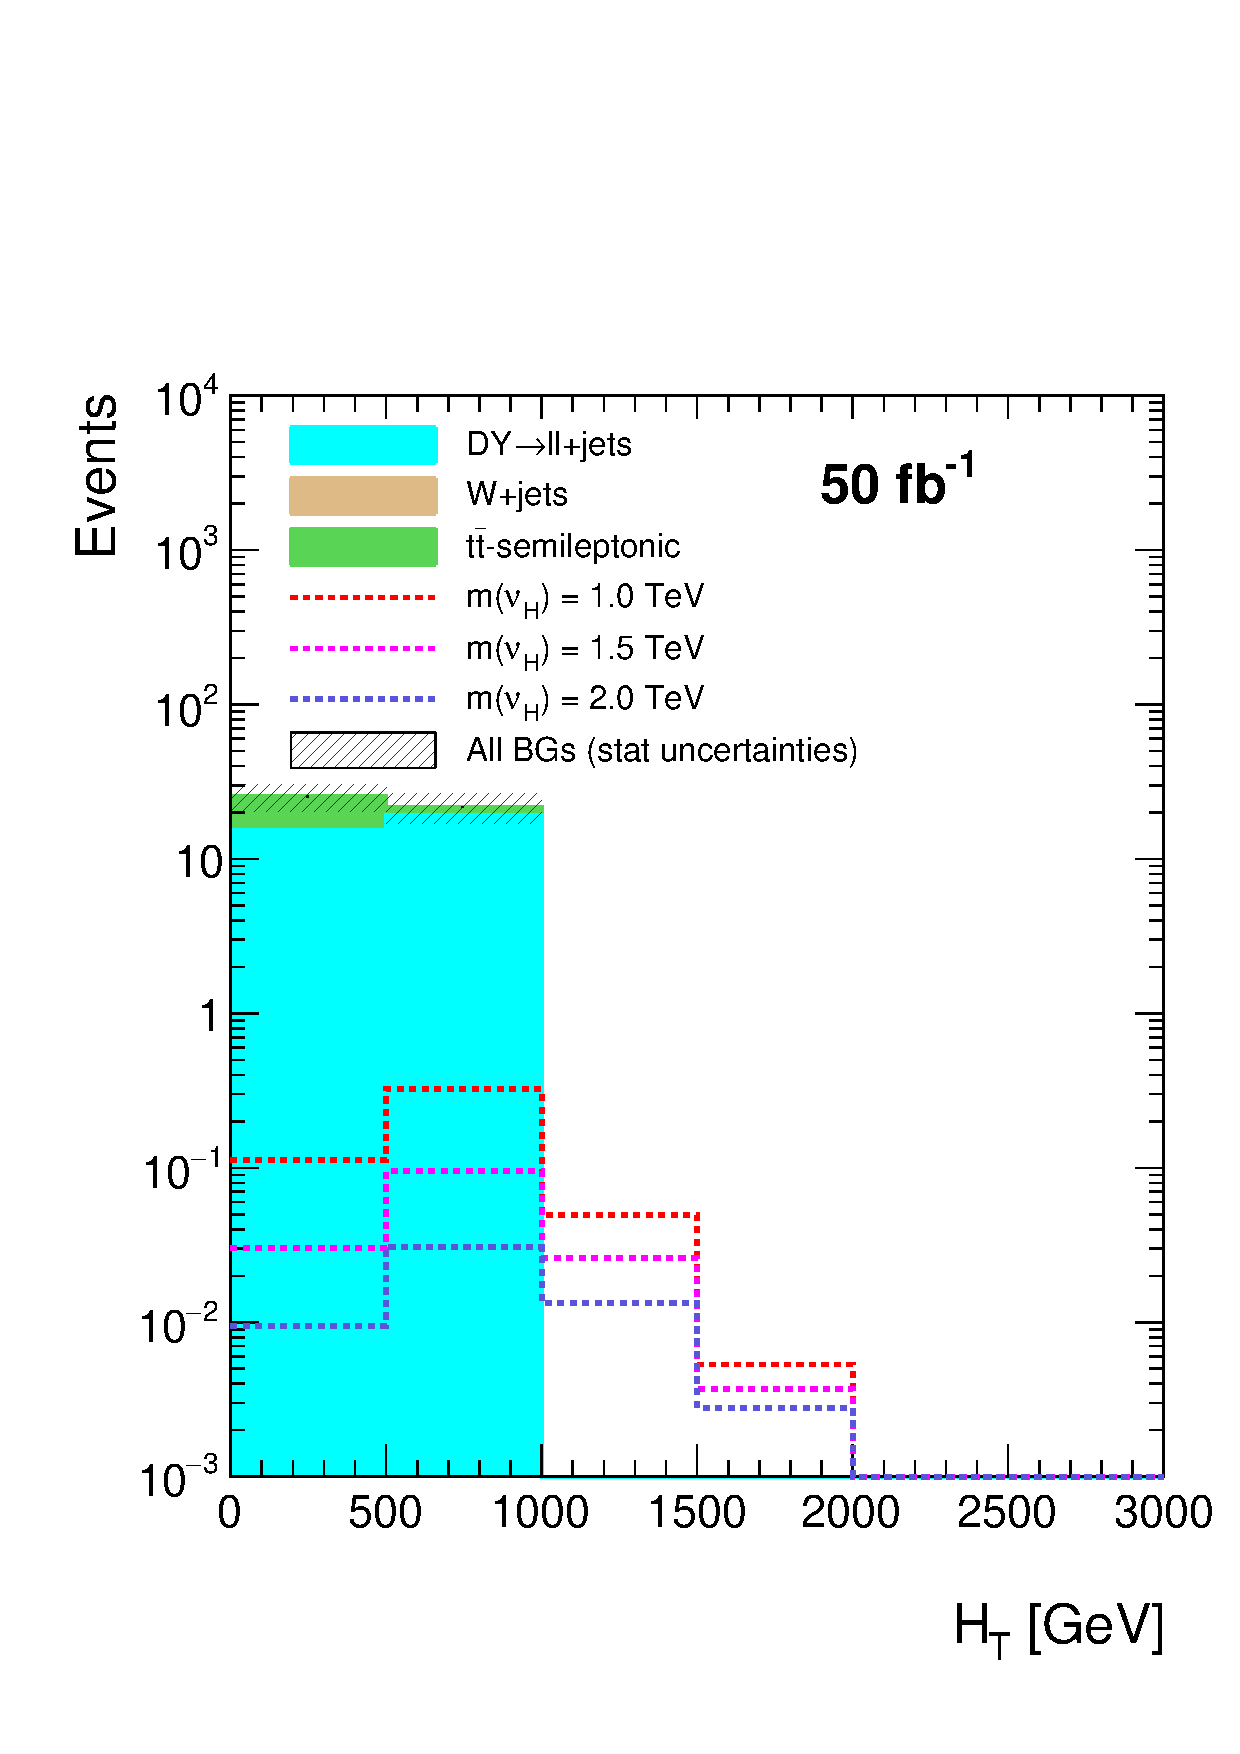
\includegraphics[width=\linewidth]{StackPlots/HT_2taus_met60_50ifb.pdf}
\caption{Stack plot of $H_{T}$ requiring two taus in the event and with $\slashed{E}_{T} > 60$}
\label{fig: HT2tausMet60}
\end{figure}

\begin{figure}
\centering
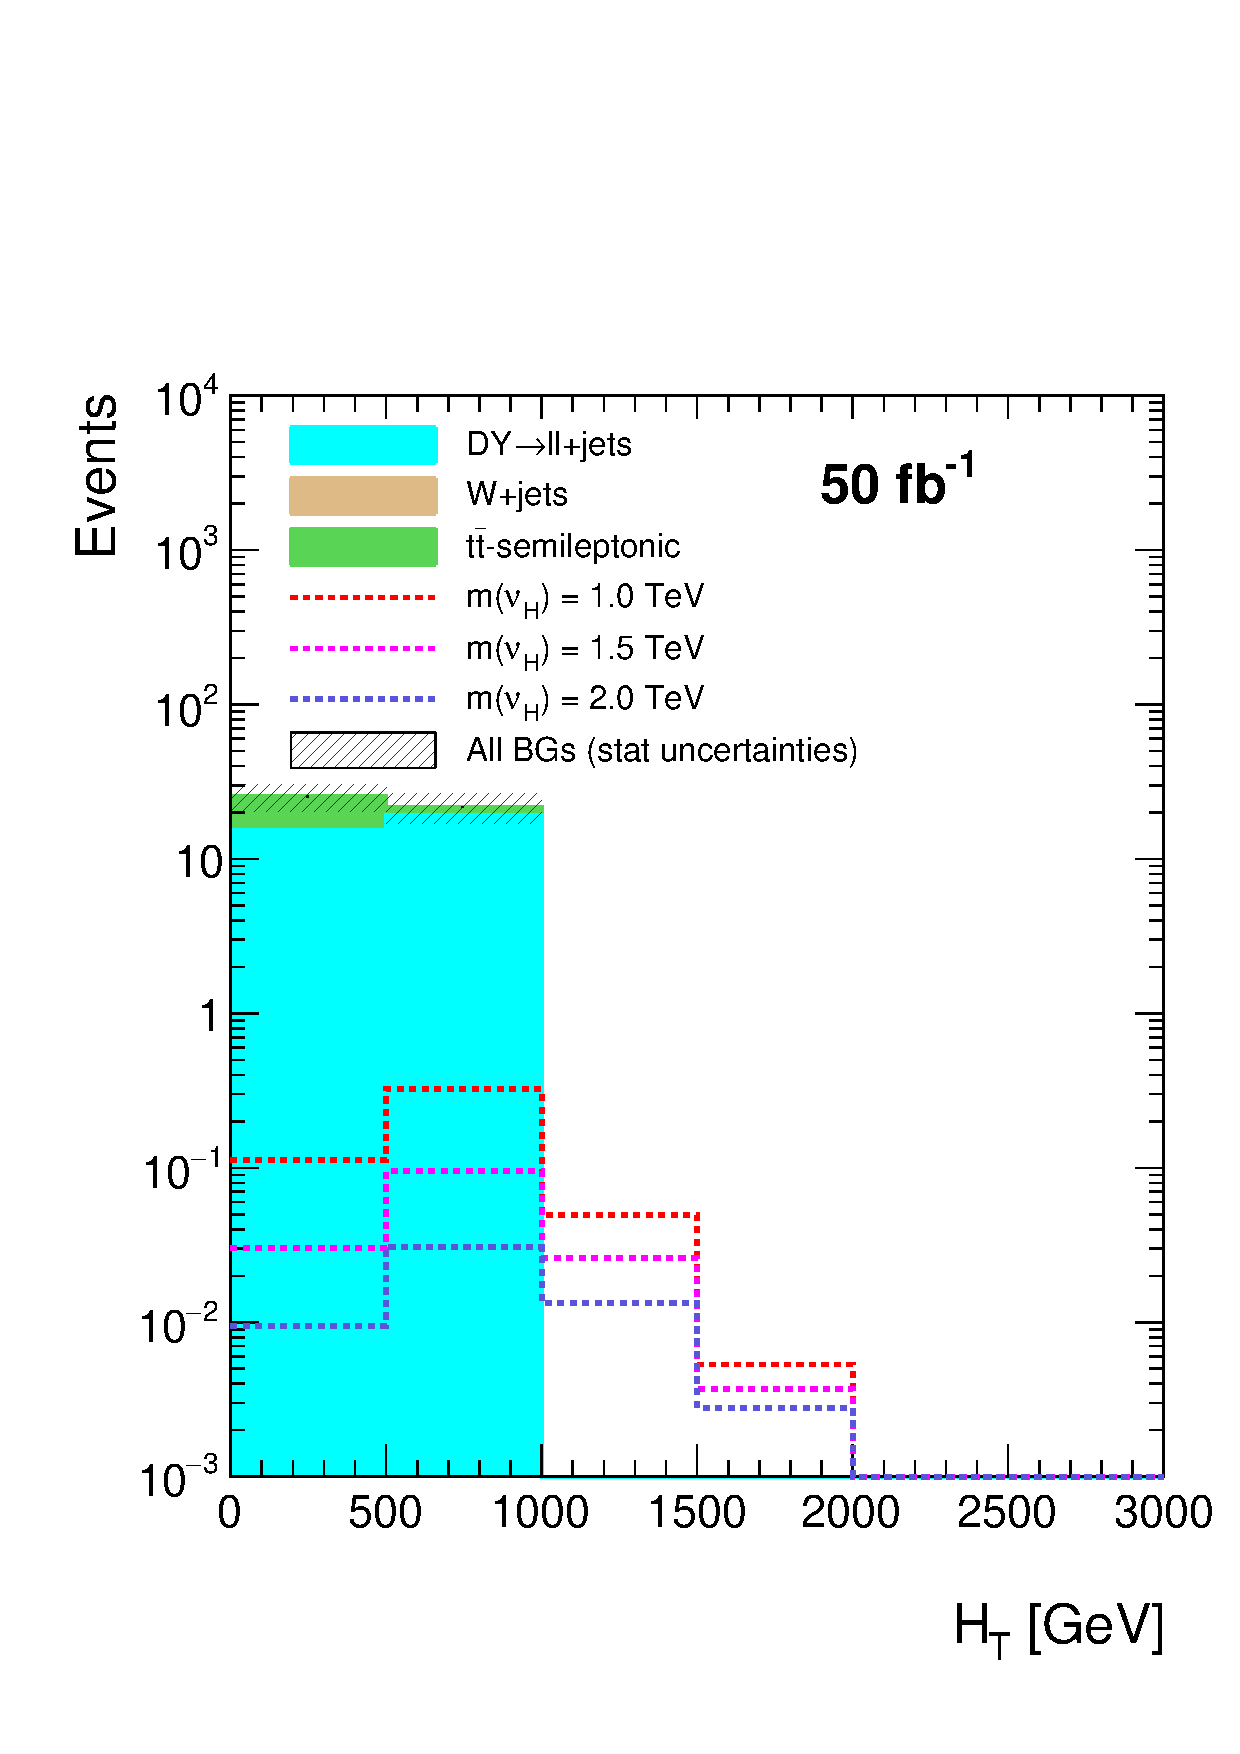
\includegraphics[width=\linewidth]{StackPlots/HT_2taus_met60_50ifb.pdf}
\caption{Stack plot of $\slashed{E_{T}}$ requiring only one tau in the event and with $\slashed{E}_{T} > 60$}
\label{fig: MET1tauMet60}
\end{figure}

\begin{figure}
\centering
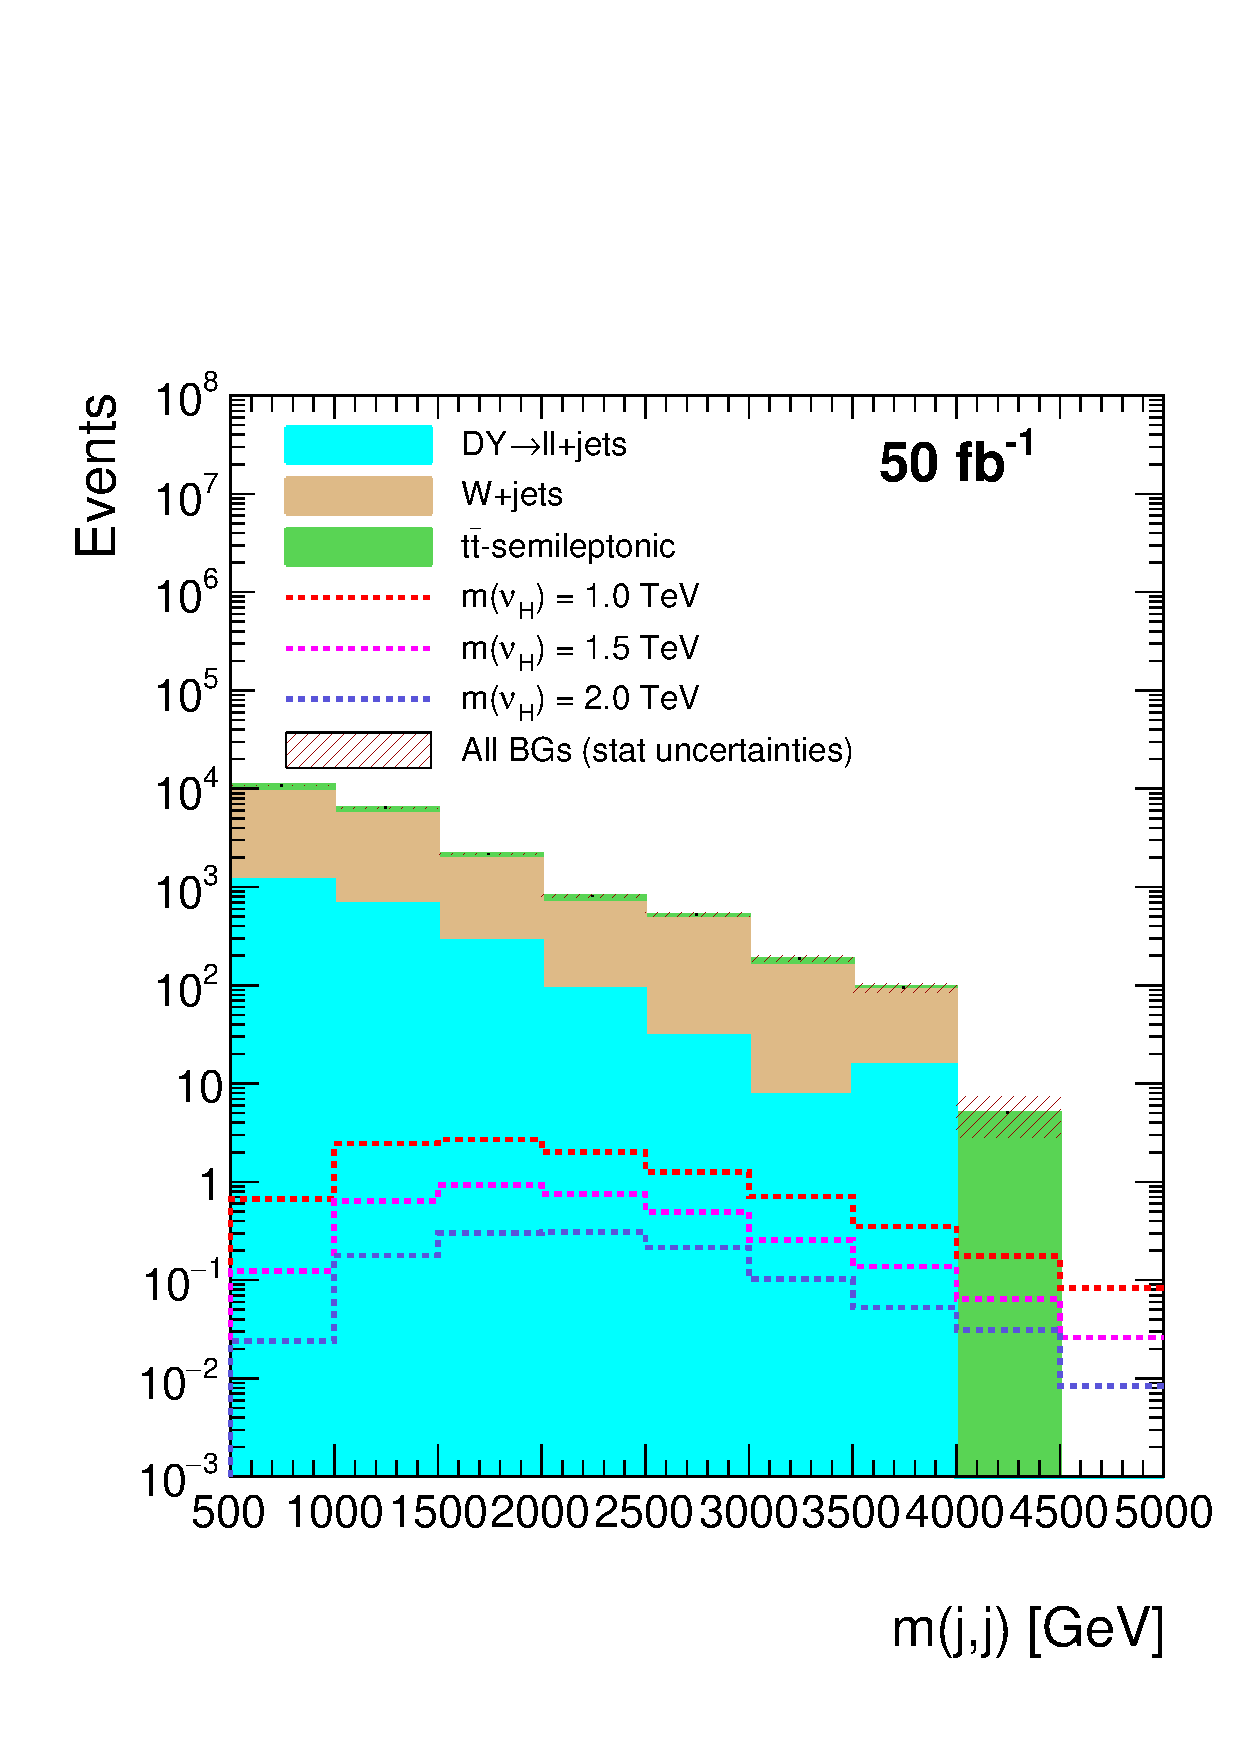
\includegraphics[width=\linewidth]{StackPlots/mjj_1Tau_met60_50ifb.pdf}
\caption{Stack plot of Di-Jet mass requiring only one tau in the event and with $\slashed{E}_{T} > 60$}
\label{fig: mjj1tauMet60}
\end{figure}

\begin{figure}
\centering
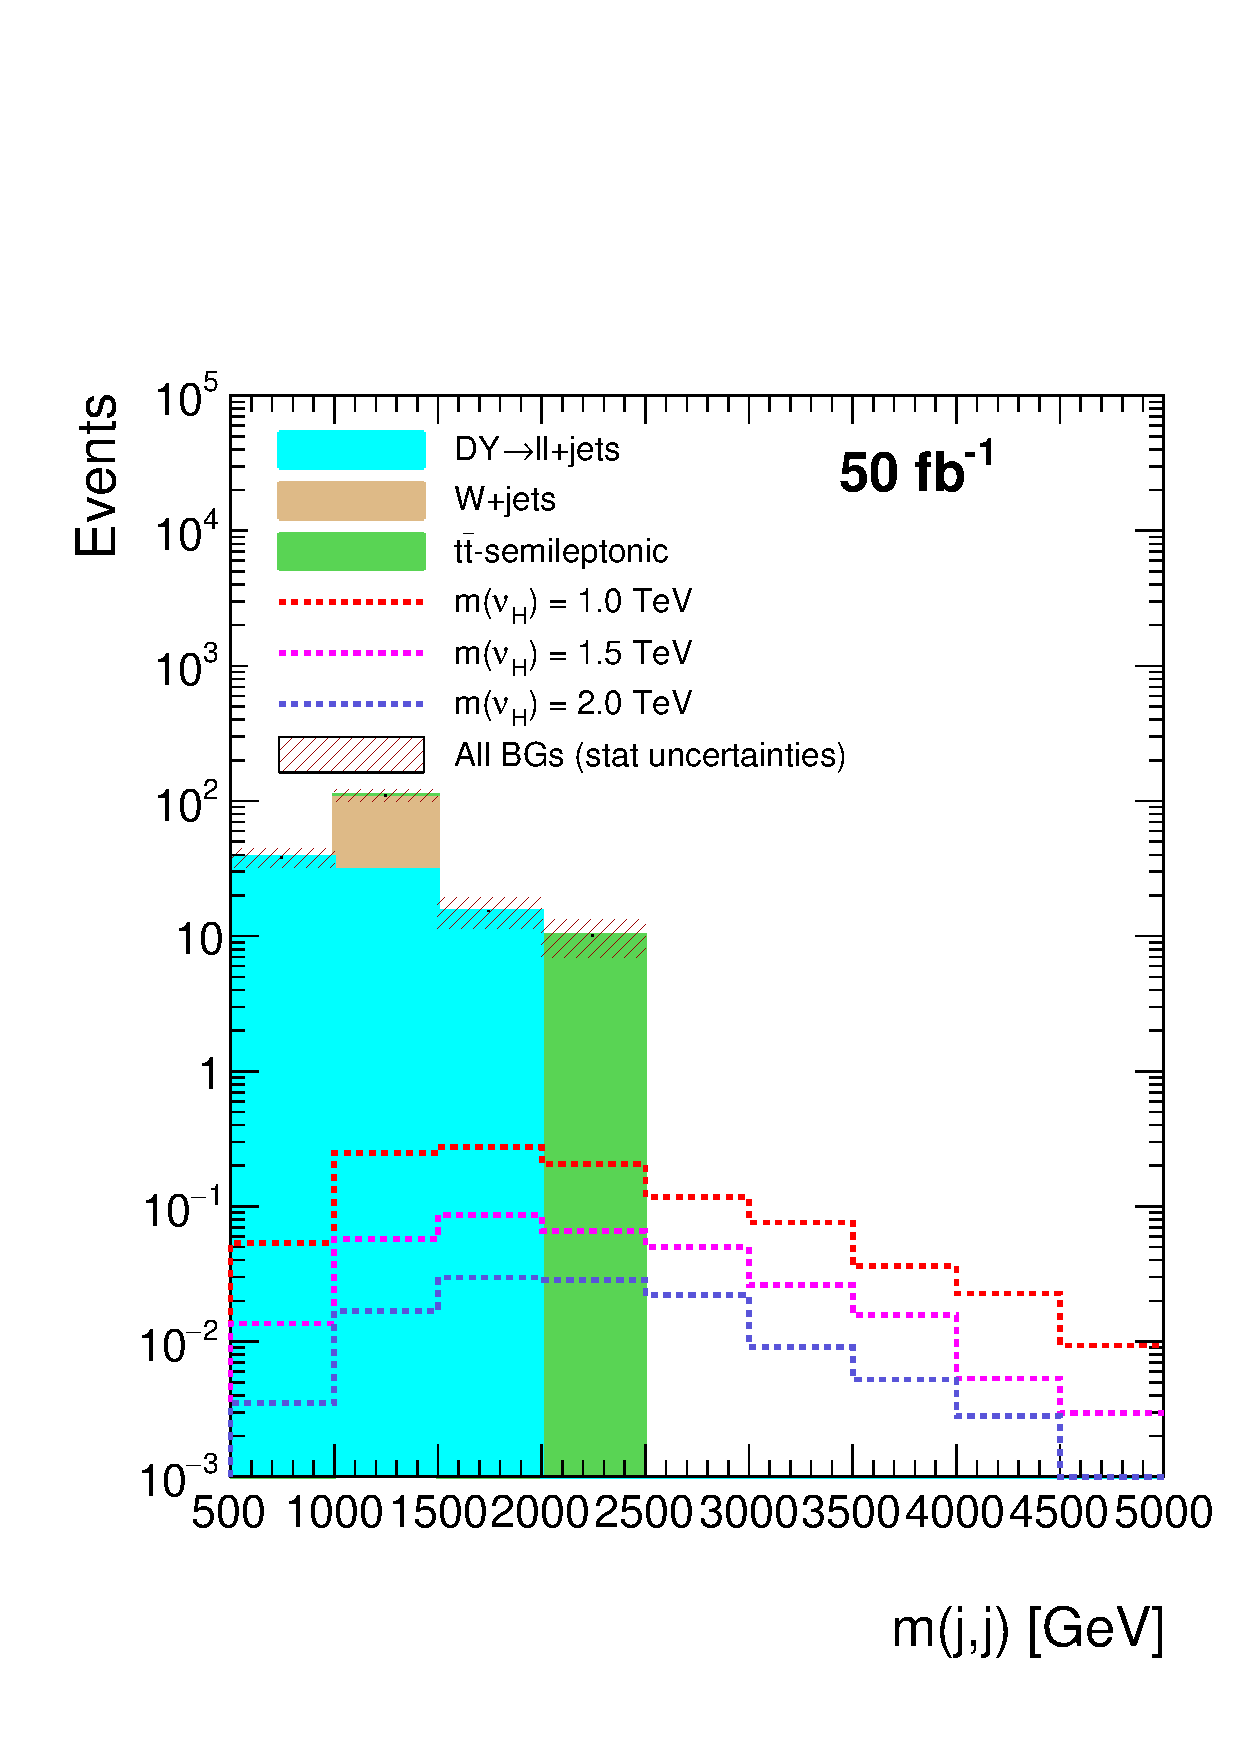
\includegraphics[width=\linewidth]{StackPlots/mjj_2taus_met50_50ifb.pdf}
\caption{Stack plot of Di-Jet mass requiring two taus in the event and with $\slashed{E}_{T} > 50$}
\label{fig: mjj2tauMet50}
\end{figure}

\begin{figure}
\centering
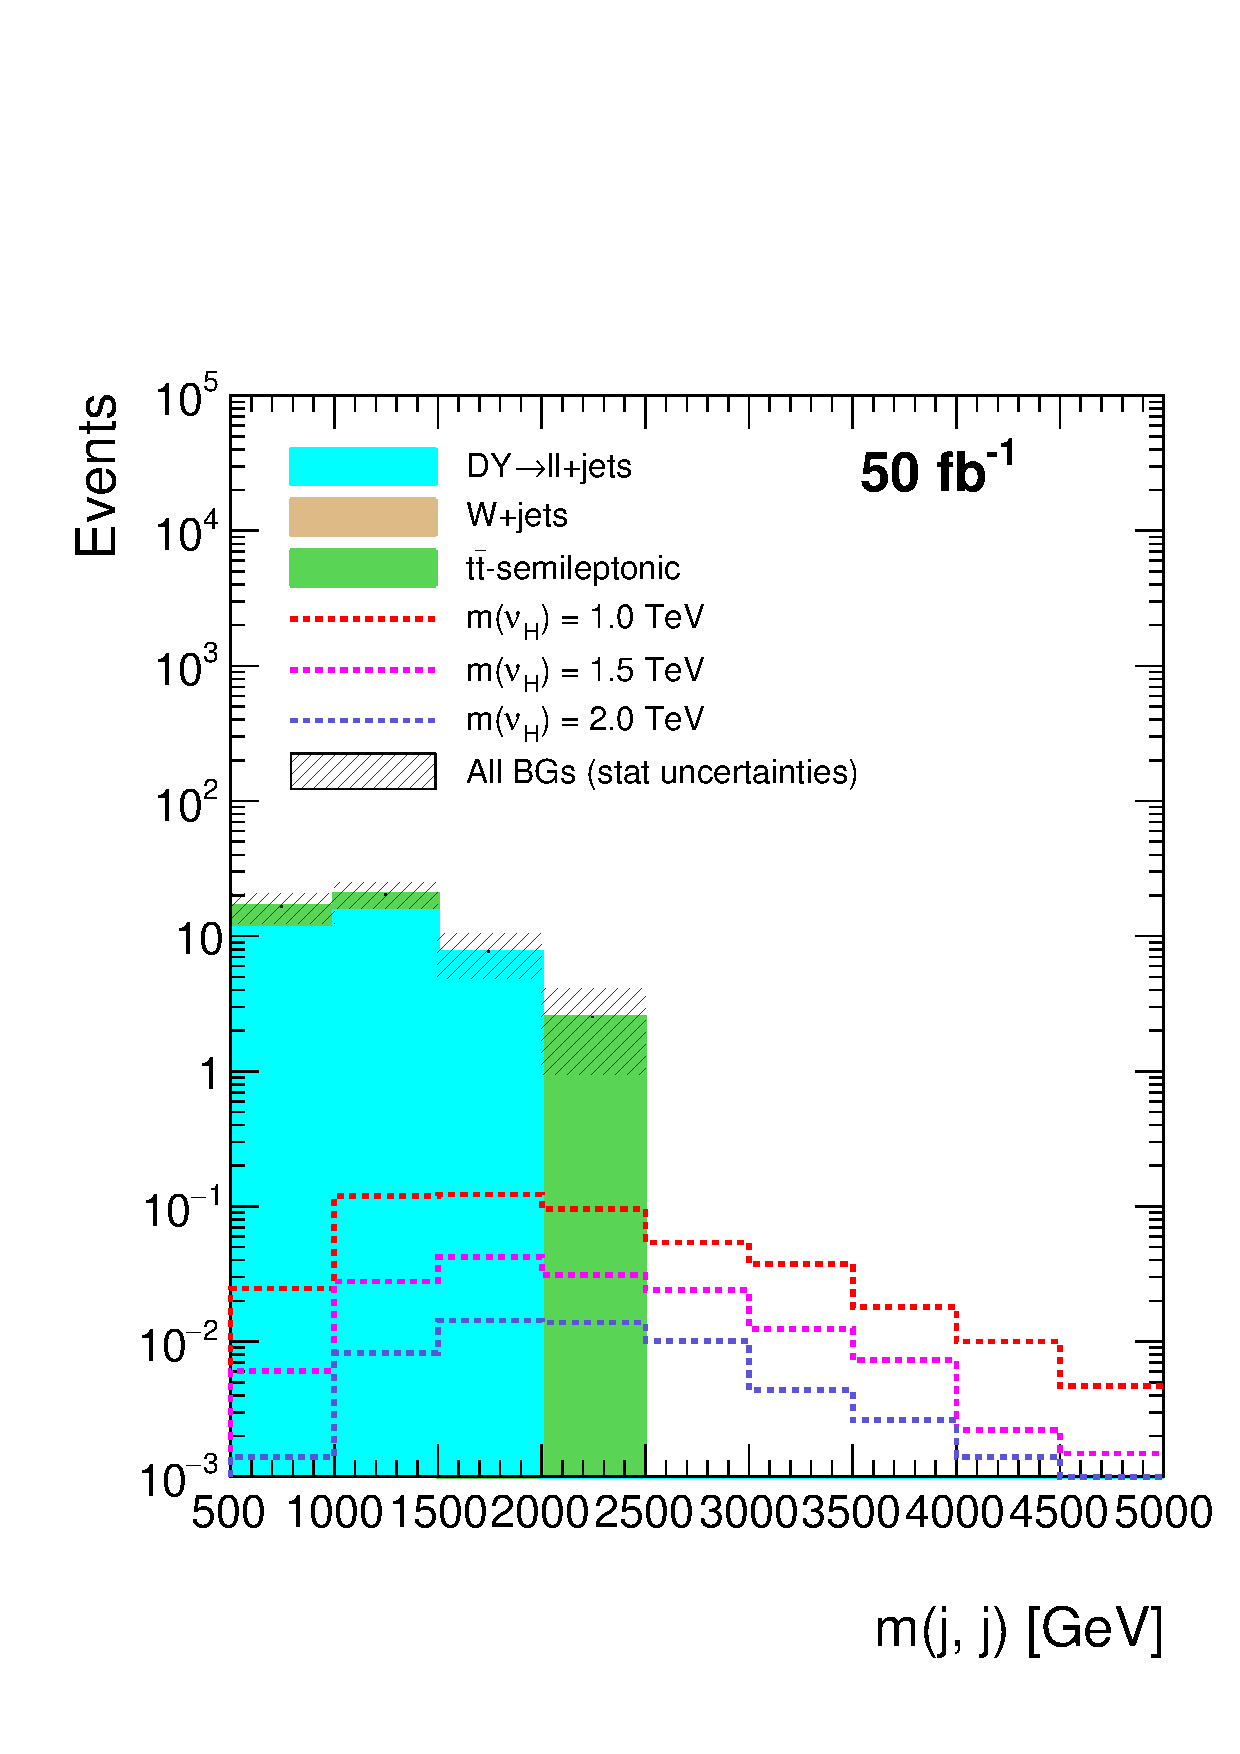
\includegraphics[width=\linewidth]{StackPlots/mjj_2taus_met60_50ifb.pdf}
\caption{Stack plot of Di-Jet mass requiring two taus in the event and with $\slashed{E}_{T} > 60$}
\label{fig: mjj2tauMet60}
\end{figure}

\begin{figure}
\centering
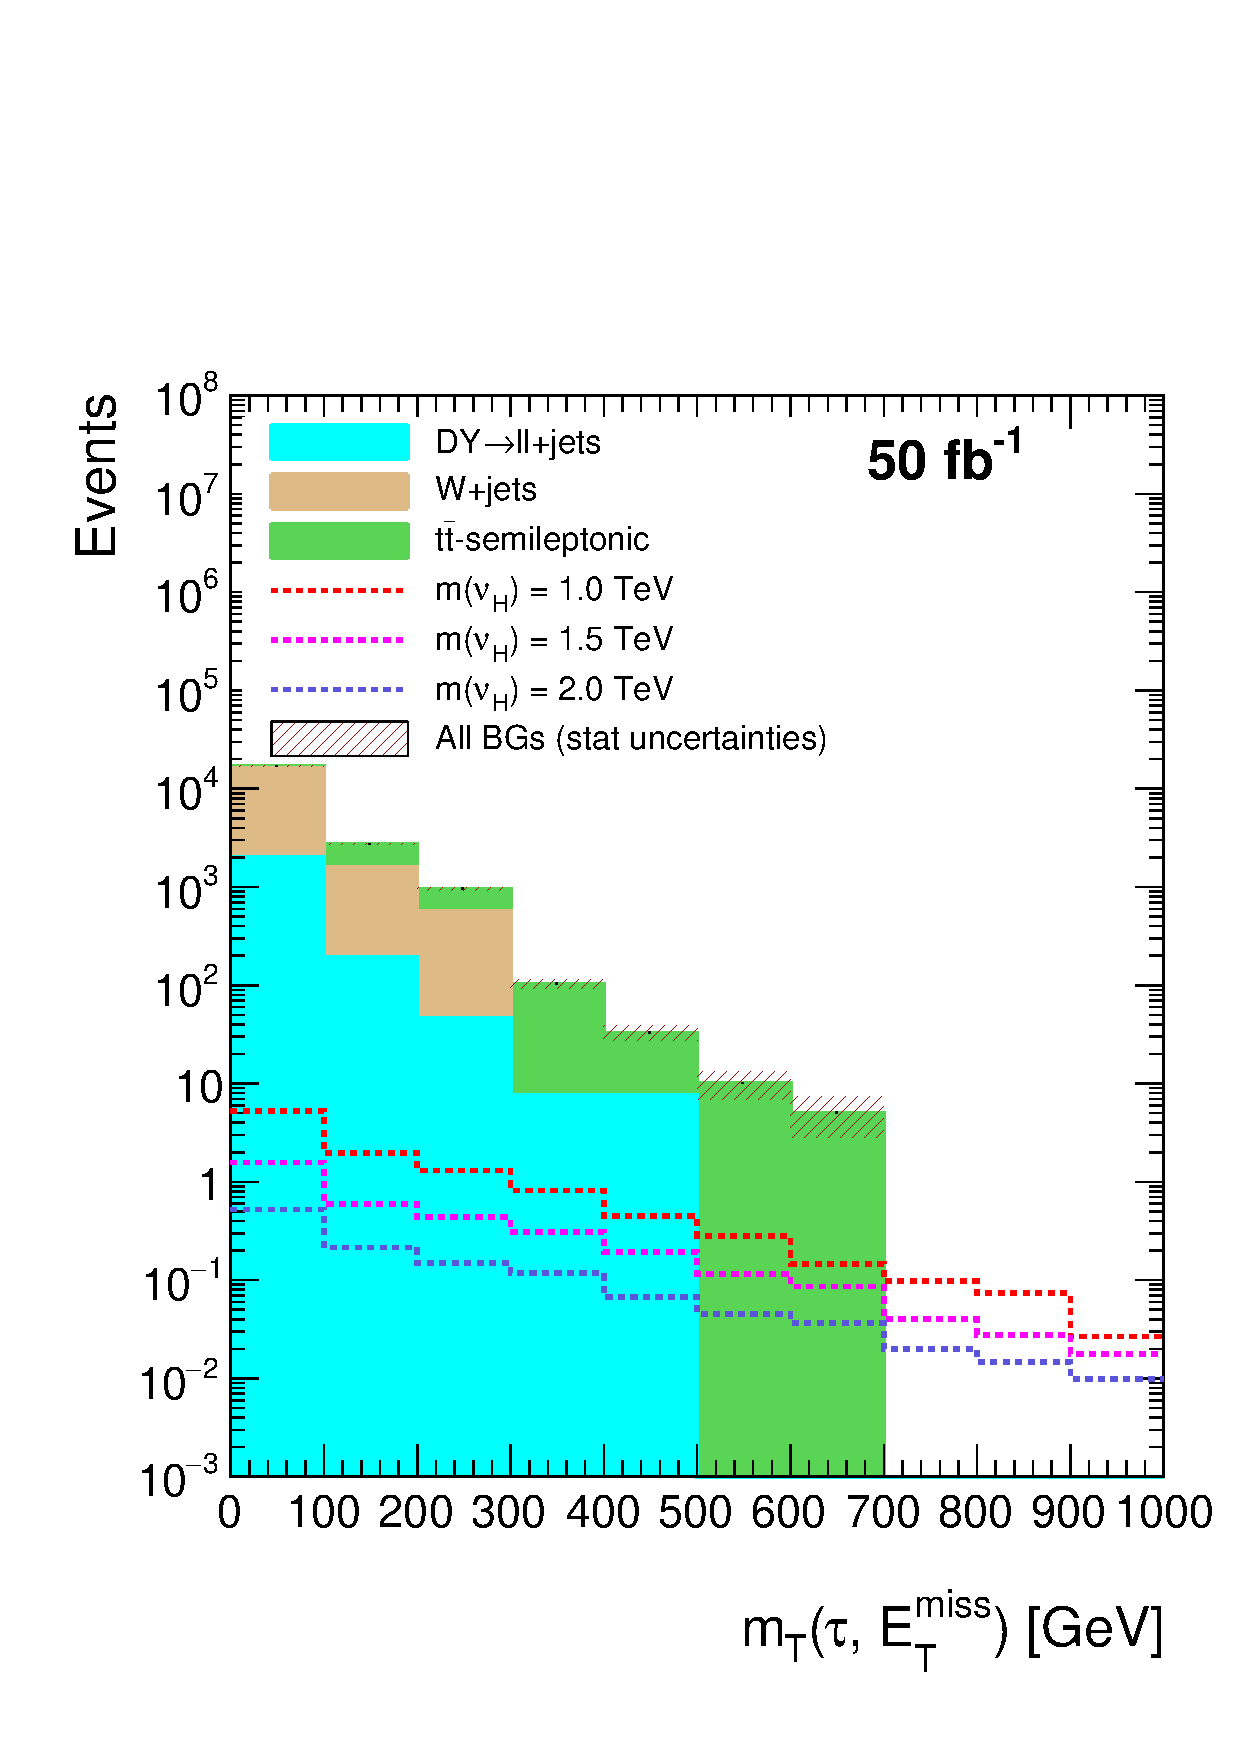
\includegraphics[width=\linewidth]{StackPlots/mT_1Tau_met60_50ifb.pdf}
\caption{Stack plot $m_{T}$ requiring only one tau in the event and with $\slashed{E}_{T} > 60$}
\label{fig: mjj2tauMet50}
\end{figure}

\begin{figure}
\centering
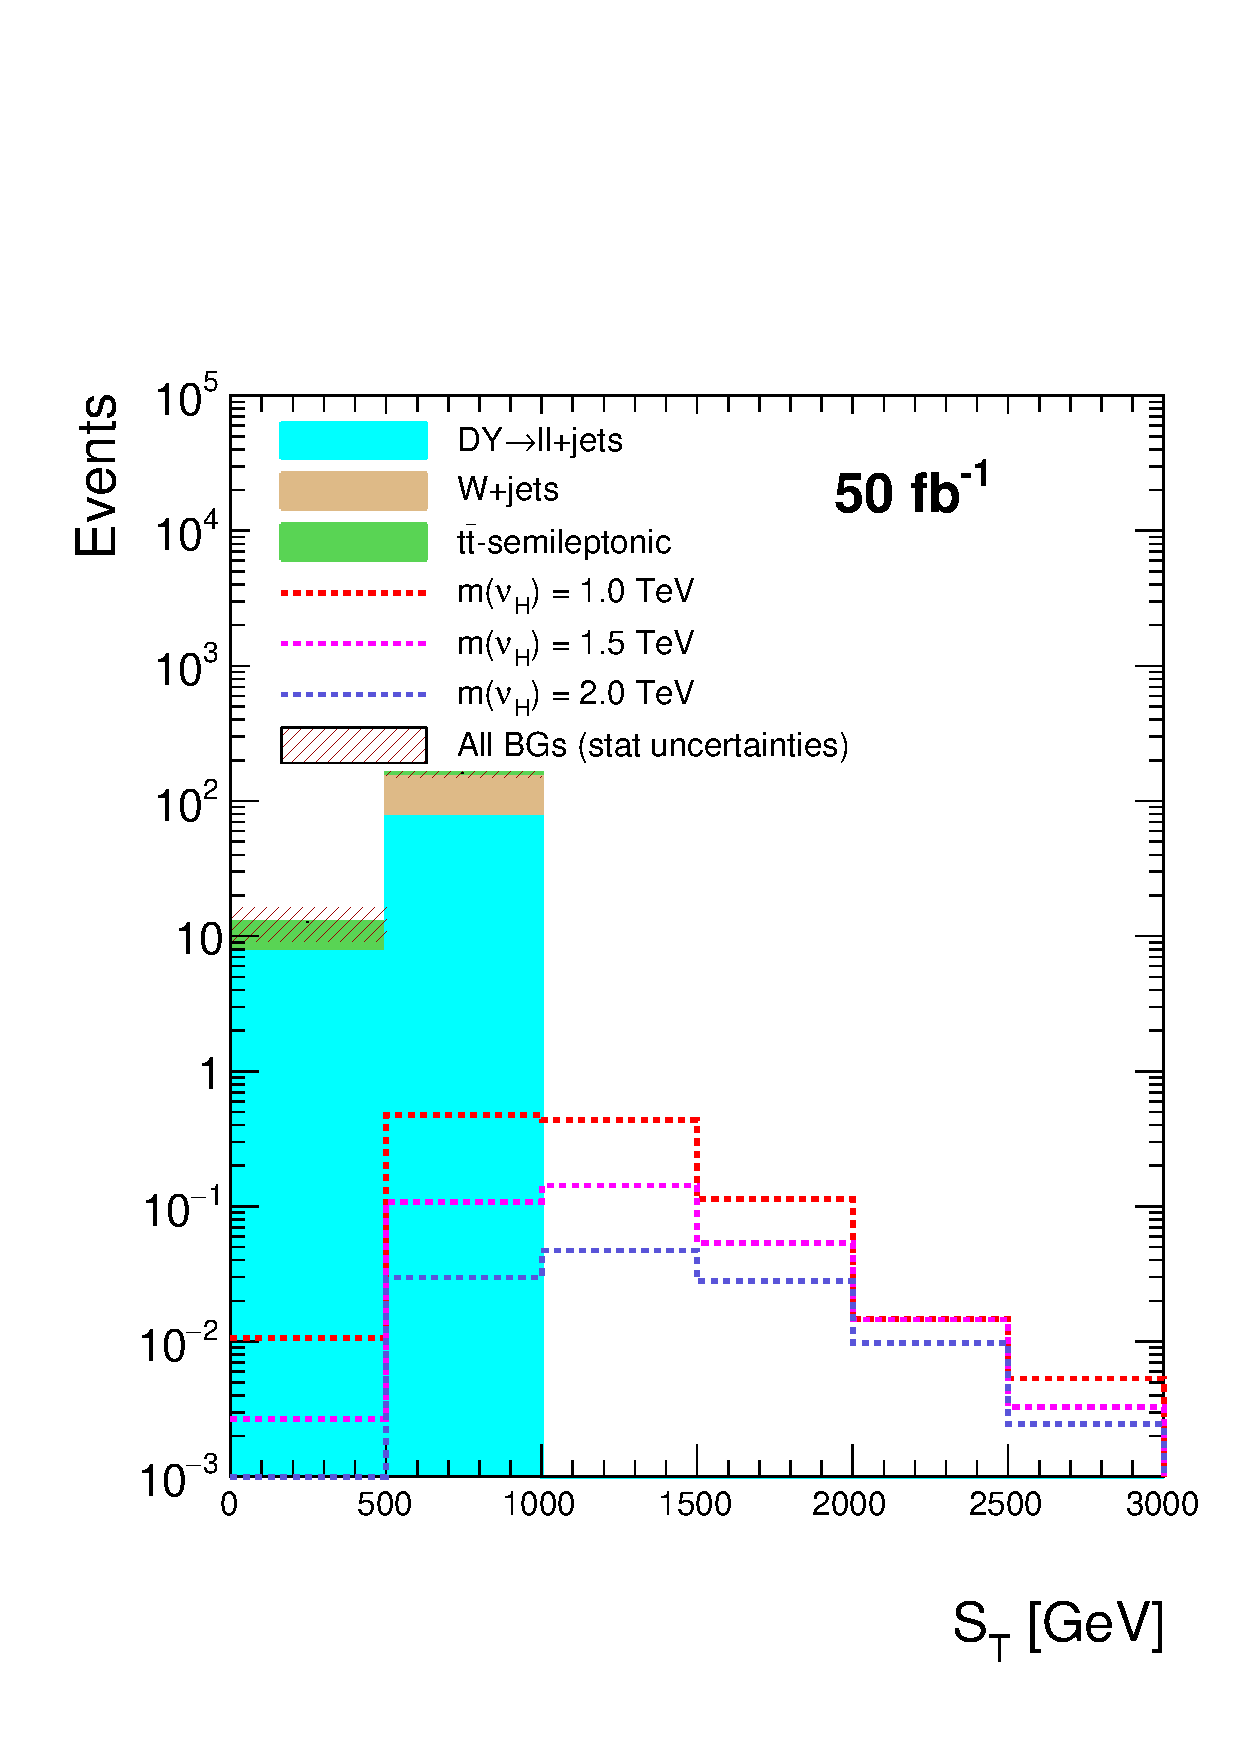
\includegraphics[width=\linewidth]{StackPlots/ST_2taus_met50_50ifb.pdf}
\caption{Stack plot of $S_{T}$ requiring two taus in the event and with $\slashed{E}_{T} > 50$}
\label{fig: HT2tausMet60}
\end{figure}


\begin{figure}
\centering
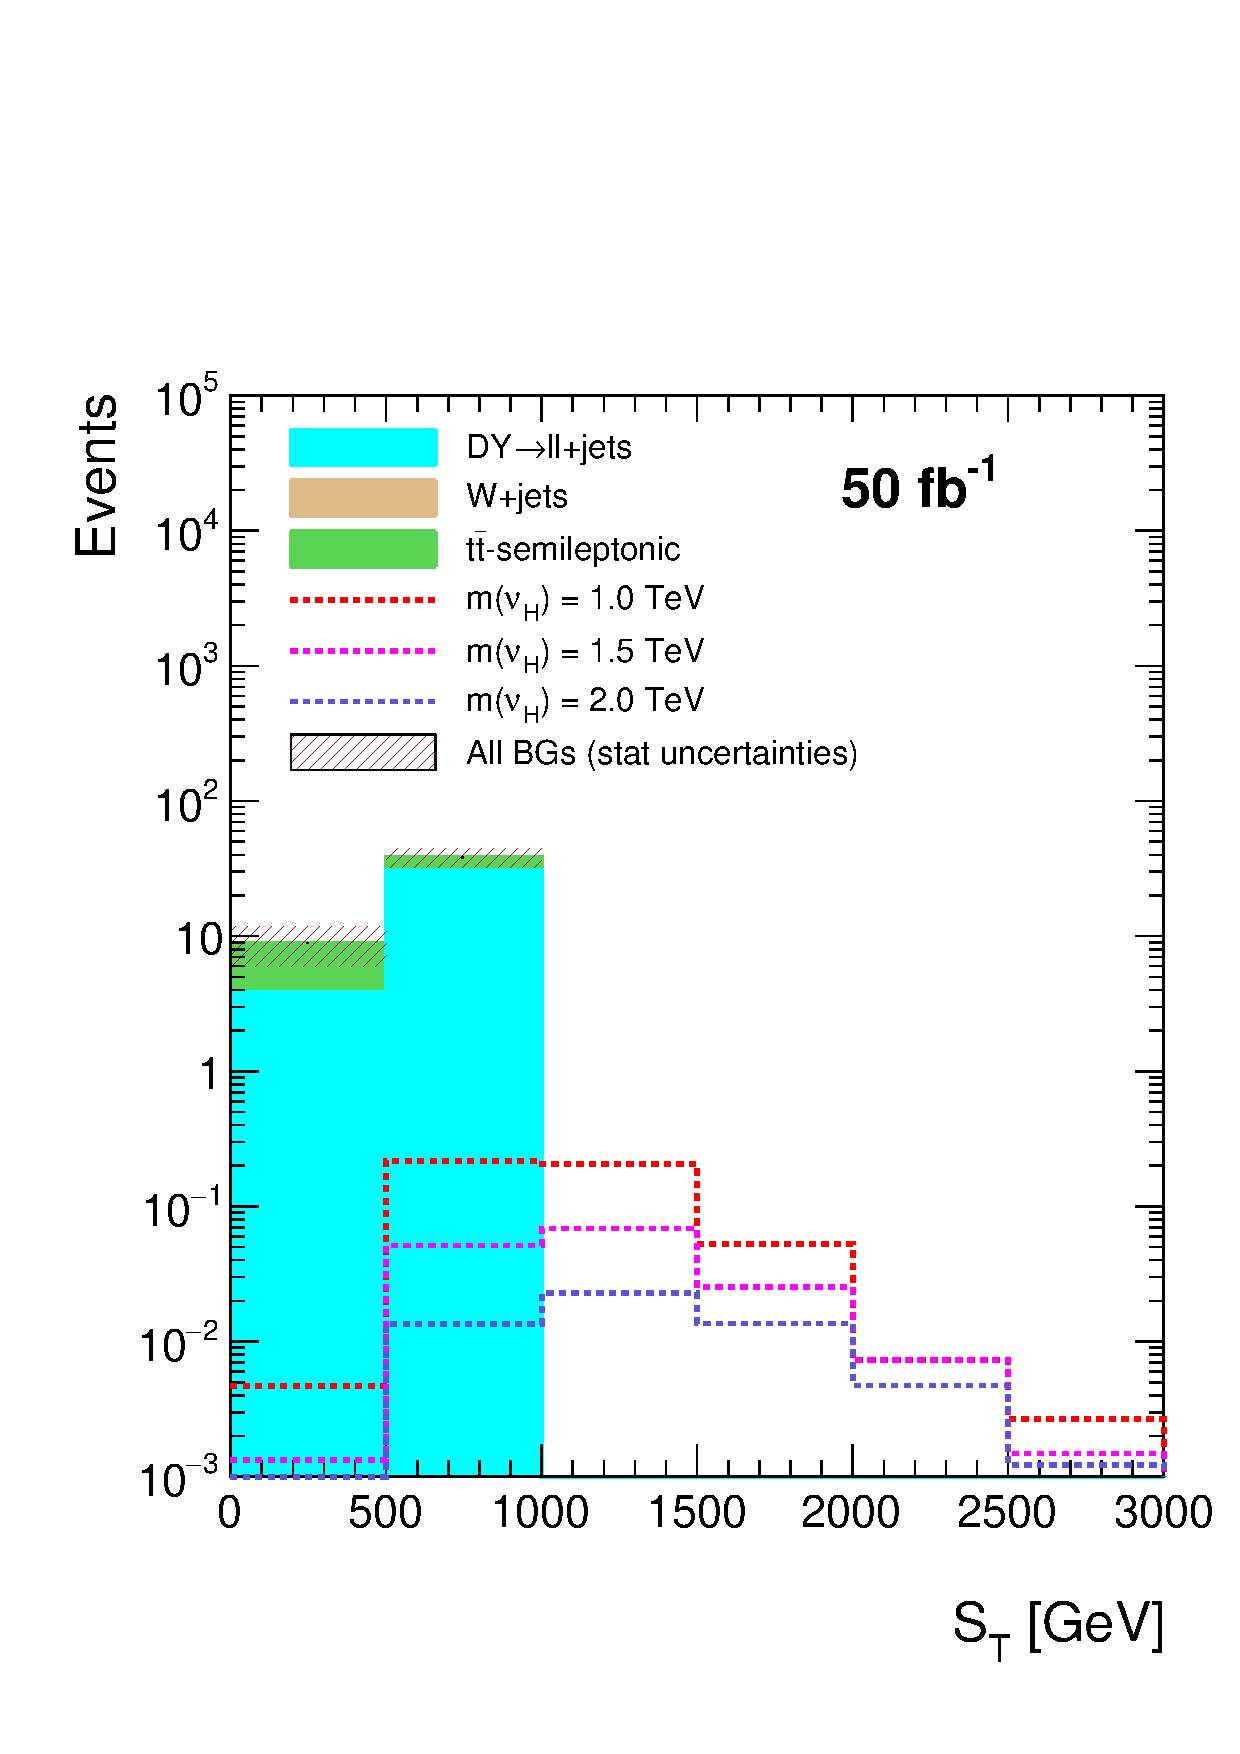
\includegraphics[width=\linewidth]{StackPlots/ST_2taus_met60_50ifb.pdf}
\caption{Stack plot of $S_{T}$ requiring two taus in the event and with $\slashed{E}_{T} > 60$}
\label{fig: HT2tausMet60}
\end{figure}












%----------------------------------------------------------------------------------------
%	APÉNDICES
%----------------------------------------------------------------------------------------

%\addtocontents{toc}{\vspace{2em}} % Agrega espacios en la toc

%\appendix % Los siguientes capítulos son apéndices

\begin{appendices}

%  Incluye los apéndices en el folder de apéndices

%\include{Apendices/Ap}
\thispagestyle{empty}
\chapter{Same Chirality Fields Terms} \label{app: samechirality}

A field $\psi$ can be decomposed in its chiral components

$$ \psi = \psi_{R} + \psi_{L} $$

where 

$$ \psi_{R} = \frac{1}{2}\left(1 + \gamma^{5}\right)\psi $$

$$ \psi_{L} = \frac{1}{2}\left(1 - \gamma^{5}\right)\psi $$

where $\gamma^{5}$ is the fifth Dirac matrix. In a similar way the fields $\bar{\psi_{R}}$ and $\bar{\psi_{L}}$ are defined as  

$$ \bar{\psi_{R}} = \frac{1}{2}\bar{\psi}\left(1 - \gamma^{5}\right) $$

$$ \bar{\psi_{L}} = \frac{1}{2}\bar{\psi}\left(1 + \gamma^{5}\right) $$

Taking into account the previous definitions, the term $\bar{\psi_{R}}\psi_{R}$ would be

$$\frac{1}{4}\bar{\psi}\left(1 - \gamma^{5}\right)\left(1+\gamma^{5}\right)\psi$$

Remebering the property $\left(\gamma^{5}\right)^{2} = 1$, the term $\left(1 - \gamma^{5}\right)\left(1+\gamma^{5}\right)$ would be zero.

A similar analysis can be performed of the the field with left chirality to obtain the same conclusion. These analysis leads to the conclude that $\bar{\psi_{R}}\psi_{R} = \bar{\psi_{L}}\psi_{L} = 0$. 




%\include{Apendices/AppendixC}

%\addtocontents{toc}{\vspace{2em}} % Agrega espacio en la toc

\end{appendices}


%----------------------------------------------------------------------------------------
%	BIBLIOGRAFÍA
%----------------------------------------------------------------------------------------
\backmatter
%\nocite{*}
%\bibliographystyle{plain}
%\bibliography{bibliografía.bib} %Aquí ponen el nombre del archivo .bib


\begin{thebibliography}{10}

\bibitem {Detectores}Particle Data Group, Olive, K. A. et al. , Chin.Phys. C38, 090001 (2014)


\bibitem{Super-Kamiokande} Fukuda, S. et al. (2003) Nuclear Instruments and Methods in Physics Research A 501 (2003) 418–462

\bibitem{KamLAND} Decowski, M. (2016). KamLAND's precision neutrino oscillation measurements. Nuclear Physics B, 908, pp.52-61.

\bibitem{K2K} K2K Collaboration: Aliu, E. et al (2005). Evidence for Muon Neutrino Oscillation in an Accelerator-Based Experiment. Physical Review Letters, 94(8).

\bibitem {Experimentos}Nakamura, K. et al. (2010) (Particle Data Group), J. Phys. G 37, 075021 (2010) 

\bibitem {See-saw} Deppisch, F., Bhupal Dev, P., \& Pilaftsis, A. (2015). Neutrinos and collider physics. New Journal Of Physics, 17(7), 075019. http://dx.doi.org/10.1088/1367-2630/17/7/075019

\bibitem {LEP} Abdesslam, A. et al. (2014) Type II Seesaw Higgsology and LEP/LHC constraints. arXiv:1411.5645 [hep-ph]

\bibitem {CMS ATLAS} Khachatryan, V., Sirunyan, A., Tumasyan, A., Adam, W., Asilar, E., \& Bergauer, T. et al. (2016). Search for heavy Majorana neutrinos in $e\pm e\pm +$ jets and $e\pm$ $\mu \pm +$ jets events in proton-proton collisions at s = 8 $\sqrt{s}=8$ TeV. Journal Of High Energy Physics, 2016(4).

\bibitem {VBF Search} Brooke, J., Buckley, M., Dunne, P., Penning, B., Tamanas, J., \& Zgubič, M. (2016). Vector boson fusion searches for dark matter at the LHC. Physical Review D, 93(11). http://dx.doi.org/10.1103/physrevd.93.113013

\bibitem{MadGraph} Alwall, J., Herquet, M., Maltoni, F., Mattelaer, O., \& Stelzer, T. (2011). MadGraph 5: going beyond. Journal Of High Energy Physics, 2011(6). http://dx.doi.org/10.1007/jhep06(2011)128

\bibitem{Pythia}Sjöstrand, T., Ask, S., Christiansen, J., Corke, R., Desai, N., \& Ilten, P. et al. (2015). An introduction to PYTHIA 8.2. Computer Physics Communications, 191, 159-177. http://dx.doi.org/10.1016/j.cpc.2015.01.024

\bibitem{Delphes} de Favereau, J., Delaere, C., Demin, P., Giammanco, A., Lemaître, V., Mertens, A., \& Selvaggi, M. (2014). DELPHES 3: a modular framework for fast simulation of a generic collider experiment. Journal Of High Energy Physics, 2014(2). http://dx.doi.org/10.1007/jhep02(2014)057

\bibitem{ROOT} Antcheva, I., Ballintijn, M., Bellenot, B., Biskup, M., Brun, R., \& Buncic, N. et al. (2009). ROOT — A C++ framework for petabyte data storage, statistical analysis and visualization.

\bibitem{NeutrinoMass} Kim, C., \& Pevsner, A. (1993). Neutrinos in Physics and Astrophysics (1st ed.). Langhorne, PA: Harwood Academic.

\bibitem{NeutrinoMass2} Mohapatra, R., \& Pal, P. (1991). Massive neutrinos in physics and astrophysics (1st ed., pp. 31-32). Singapore: World Scientific.

\end{thebibliography}



\end{document}
